\begin{frame}[c]{Where are we? The big picture}

\begin{itemize}
\item Algorithm Selection
  \begin{itemize}
    \item Portfolios
    \item Algorithm selection (for runtime)
  \end{itemize}
  \item Design decisions:\\ Local Search + Evo. Algorithms + Machine Learning 
  \item Empirical evaluation
  \item[$\to$] AAD for ML
  \begin{itemize}
    \item[$\to$] Hyperparameter optimization and Bayesian optimization 
    \item Neural architecture search (lecture given by Prof. Hutter)
  \end{itemize}
  \item Algorithm configuration 
  \begin{itemize}
    \item Basics 
    \item State of the art 
    \item Best practices 
  \end{itemize}
  \item Combinations of algorithm selection and configurations
  \item Algorithm control 
  \item Algorithm analysis 
  \item Project announcement and questions for exam 
\end{itemize}

\end{frame}
%----------------------------------------------------------------------
%----------------------------------------------------------------------
\begin{frame}[c]{}

\huge
\centering
Bayesian Optimization and Hyperparameter Optimization

\end{frame}
%----------------------------------------------------------------------
%----------------------------------------------------------------------
\begin{frame}[c]{Learning Goals}

After this lecture, you will be able to \ldots

\begin{itemize}
  \item explain the \alert{challenges in hyperparameter optimization}
  \item efficiently optimize black box functions via \alert{Bayesian Optimization}
  \begin{itemize}
    \item discuss the advantages of different \alert{surrogate models}
    \item explain the idea of \alert{acquisition functions} to trade off exploration and exploitation
  \end{itemize}
  \item define \alert{configuration spaces}
  \item understand \alert{grey-boxes} for hyperparameter optimization (HPO)
\end{itemize}


\end{frame}
%-----------------------------------------------------------------------
%----------------------------------------------------------------------
\begin{frame}[c]{How to Optimize Black Box Functions?}

\centering
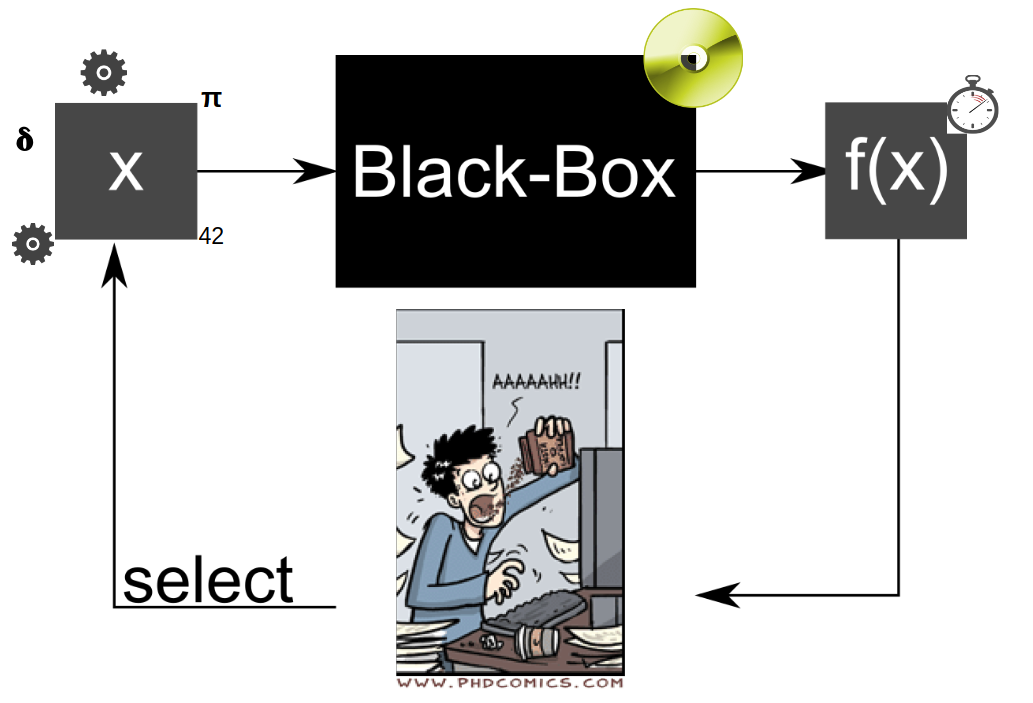
\includegraphics[width=0.7\textwidth]{images/black_box_manual_opt.png}

Only interaction: Query of function at $x$ to obtain $f(x)$

\end{frame}
%-----------------------------------------------------------------------
%----------------------------------------------------------------------
\begin{frame}[c]{How to Optimize Black Box Functions?}

\centering
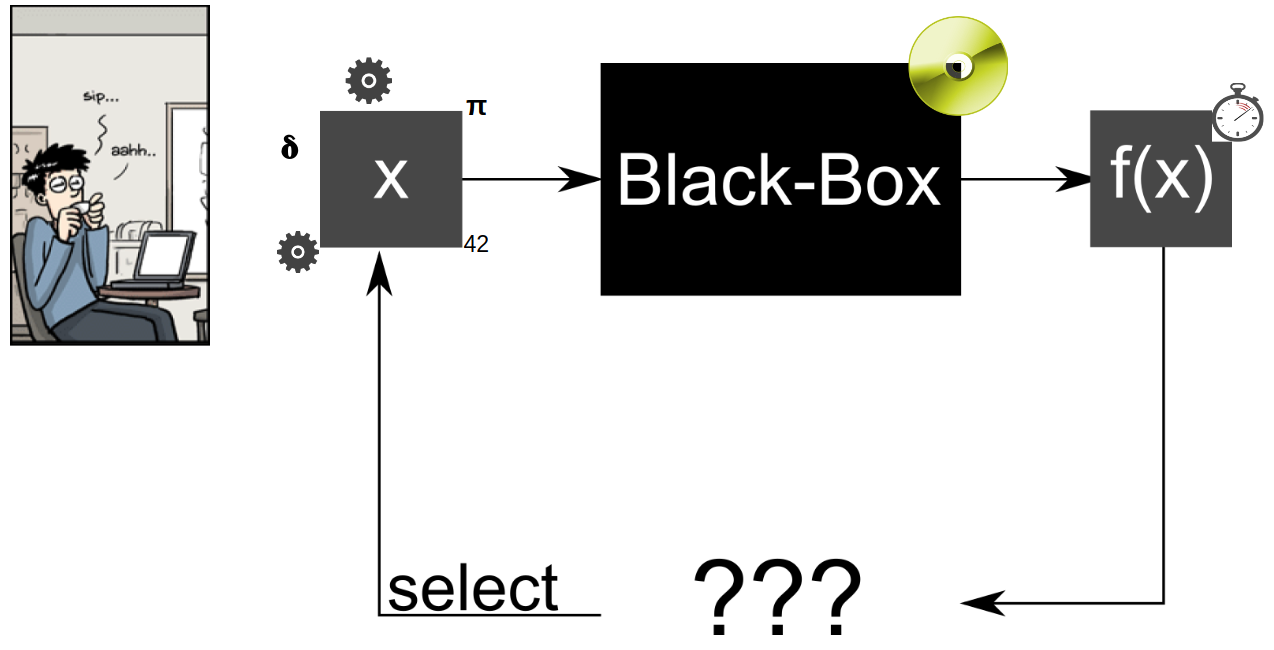
\includegraphics[width=0.9\textwidth]{images/black_box_aut_opt.png}

\end{frame}
%-----------------------------------------------------------------------
%----------------------------------------------------------------------
\begin{frame}[c]{Why Black Box Functions for AAD?}

\begin{itemize}
  \item Internals of algorithms are often not known\\
  (or well understood)
  \item Extreme: Only way of interaction is running the algorithms
\end{itemize}

\pause
\begin{block}{Example: Hyperparameter Optimization (HPO)}
Let 
\begin{itemize}
  \item $\lambda$ be the hyper-parameters of an ML algorithm $A$ with domain $\Lambda$,
  \item $D_{opt}$ be a training set which is split into $D_{train}$ and $D_{valid}$ 
  \item $\mathcal{L}(A_\lambda, D_{train}, D_{valid})$ denote the loss of $A_\lambda$ trained on $D_{train}$ and evaluated on $D_{valid}$.
\end{itemize}
The \emph{hyper-parameter optimization (HPO)} problem is to find hyper-parameter configuration that minimizes this loss:

\begin{equation}
\lambda^* \in \argmin_{\lambda \in \Lambda} \mathcal{L}(A_\lambda, D_{train}, D_{valid}) \nonumber  
\end{equation}

\end{block}

\end{frame}
%----------------------------------------------------------------------
%----------------------------------------------------------------------
\begin{frame}[c]{Challenges in HPO}
\only<1>
{%
	\centering
	
	\vspace*{2.25cm}
	
	What could be challenges in hyperparameter optimization?
	
	\bigskip
	
	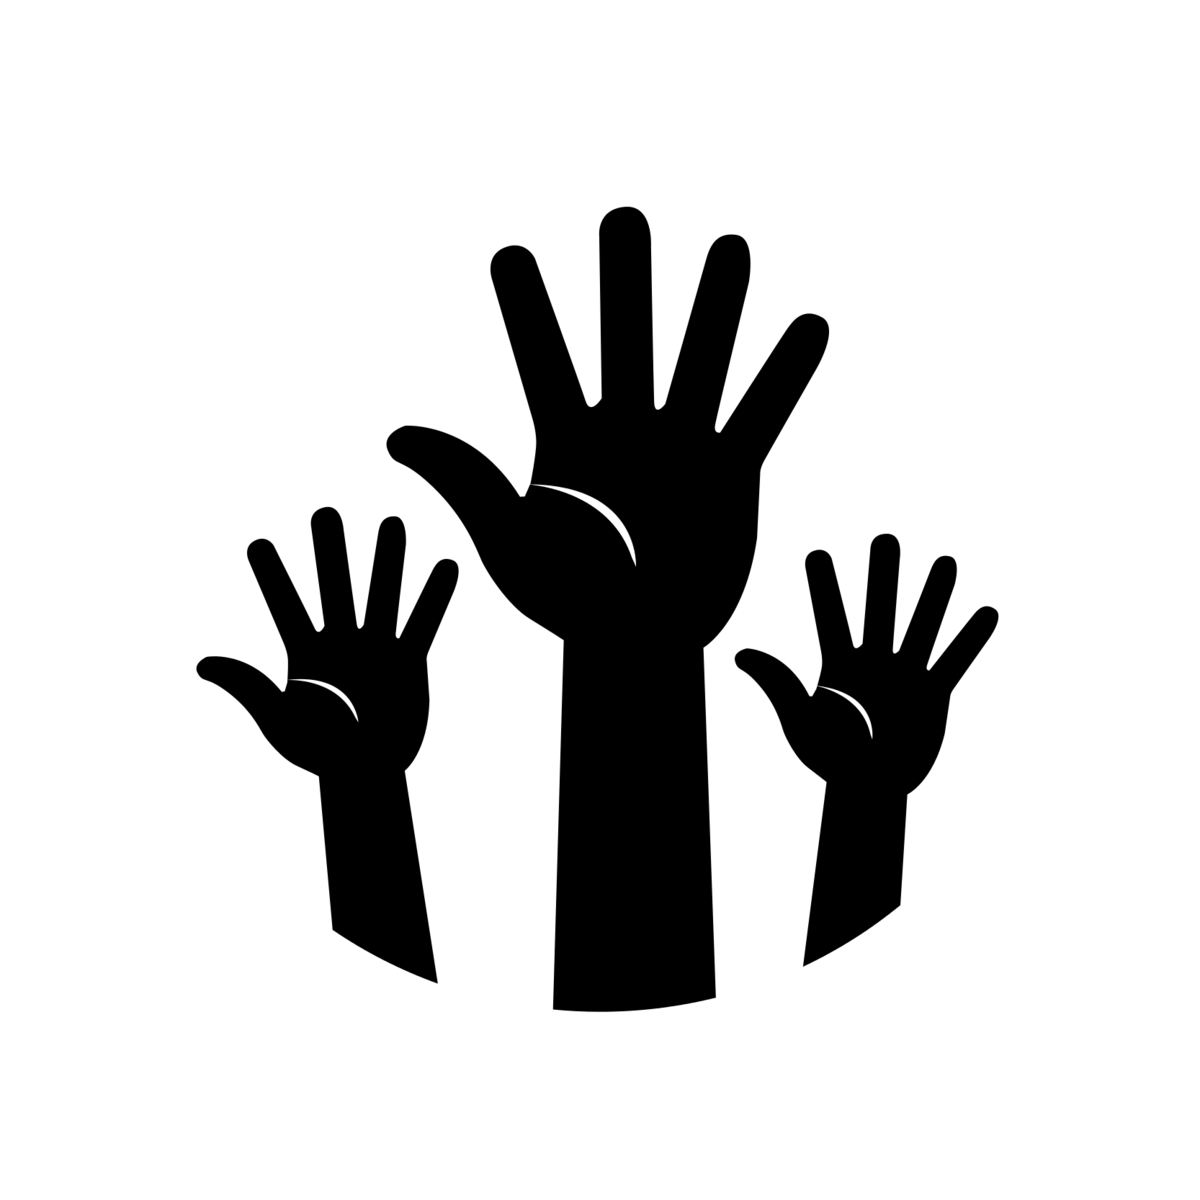
\includegraphics[width=0.2\textwidth]{images/hands.png}
}%
\pause
\begin{itemize}
  \item function evaluations are very expensive
  \begin{itemize}
    \item training a single ML-pipeline can require minutes (or even hours) 
    \item[$\leadsto$] exhaustive search is not feasible
  \end{itemize}
  \pause
  \medskip
  \item complex, structured search space
  \begin{itemize}
    \item small continuous parameter spaces already challenging to optimize
    \item typically, we talk about large configuration spaces\newline ($\gg 10$ hyper-parameters)
    \begin{itemize}
      \item typical HPO benchmarks only consider a few continuous parameters
    \end{itemize}
    \item mixed parameter types
    \item conditional structures
  \end{itemize}
  \pause
  \medskip
  \item resembles a black-box optimization problem
  \begin{itemize}
    \item Input: hyperparameter configuration
    \item Black box: ML pipeline 
    \item Output: loss
    \item Note: no gradient information available
  \end{itemize}
\end{itemize}

\end{frame}
%----------------------------------------------------------------------
%----------------------------------------------------------------------
\begin{frame}[c]{Notation}

\begin{itemize}
  \item ML-Community: 
  \begin{itemize}
    \item ``Parameters'' are part of the trained model;\\
    	  e.$\,$g., weights of a linear model;\\
    	  denoted as $\theta$
    \item ``Hyperparameters'' are parameters of the ML algorithm\\
    		e.$\,$g., $k$ of $k$-NN\\
    		denoted as $\lambda$
    \item[$\leadsto$] We are interested in optimizing $\lambda$;\\
    \item[$\leadsto$] The optimization of $\theta$ is handled by the black-box     			 
  \end{itemize}
  \pause
  \item General algorithm configuration community:
  \begin{itemize}
    \item Different notation:\\
     	  Parameters of an algorithm are denoted as $\theta$
  \end{itemize}
  \pause
  \item \alert{In the following, we use $\theta$ (and not $\lambda$) for hyperparameters of\\ ML algorithms}
\end{itemize}

\end{frame}
%-----------------------------------------------------------------------
\begin{frame}[c]{How to Optimize Black Box Functions?}

\centering
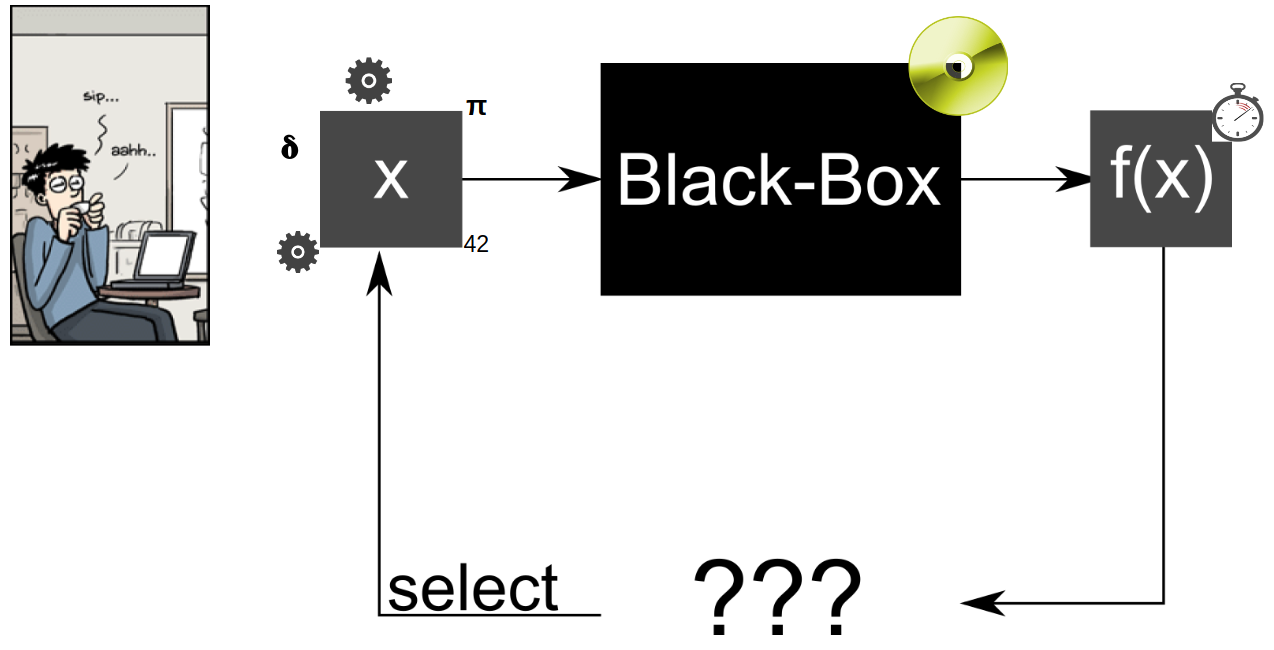
\includegraphics[width=0.9\textwidth]{images/black_box_aut_opt.png}

\end{frame}
%-----------------------------------------------------------------------
%-----------------------------------------------------------------------
\begin{frame}[c,fragile]{Grid Search \litw{Bergstra et al. '12}}

\begin{center}
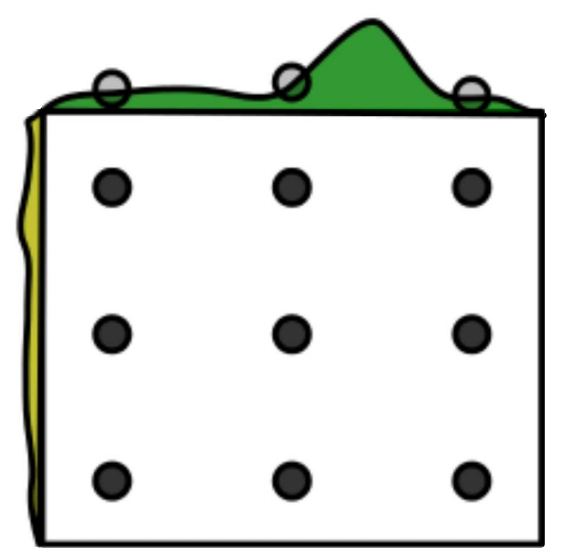
\includegraphics[width=0.28\textwidth]{plots/grid_search}%
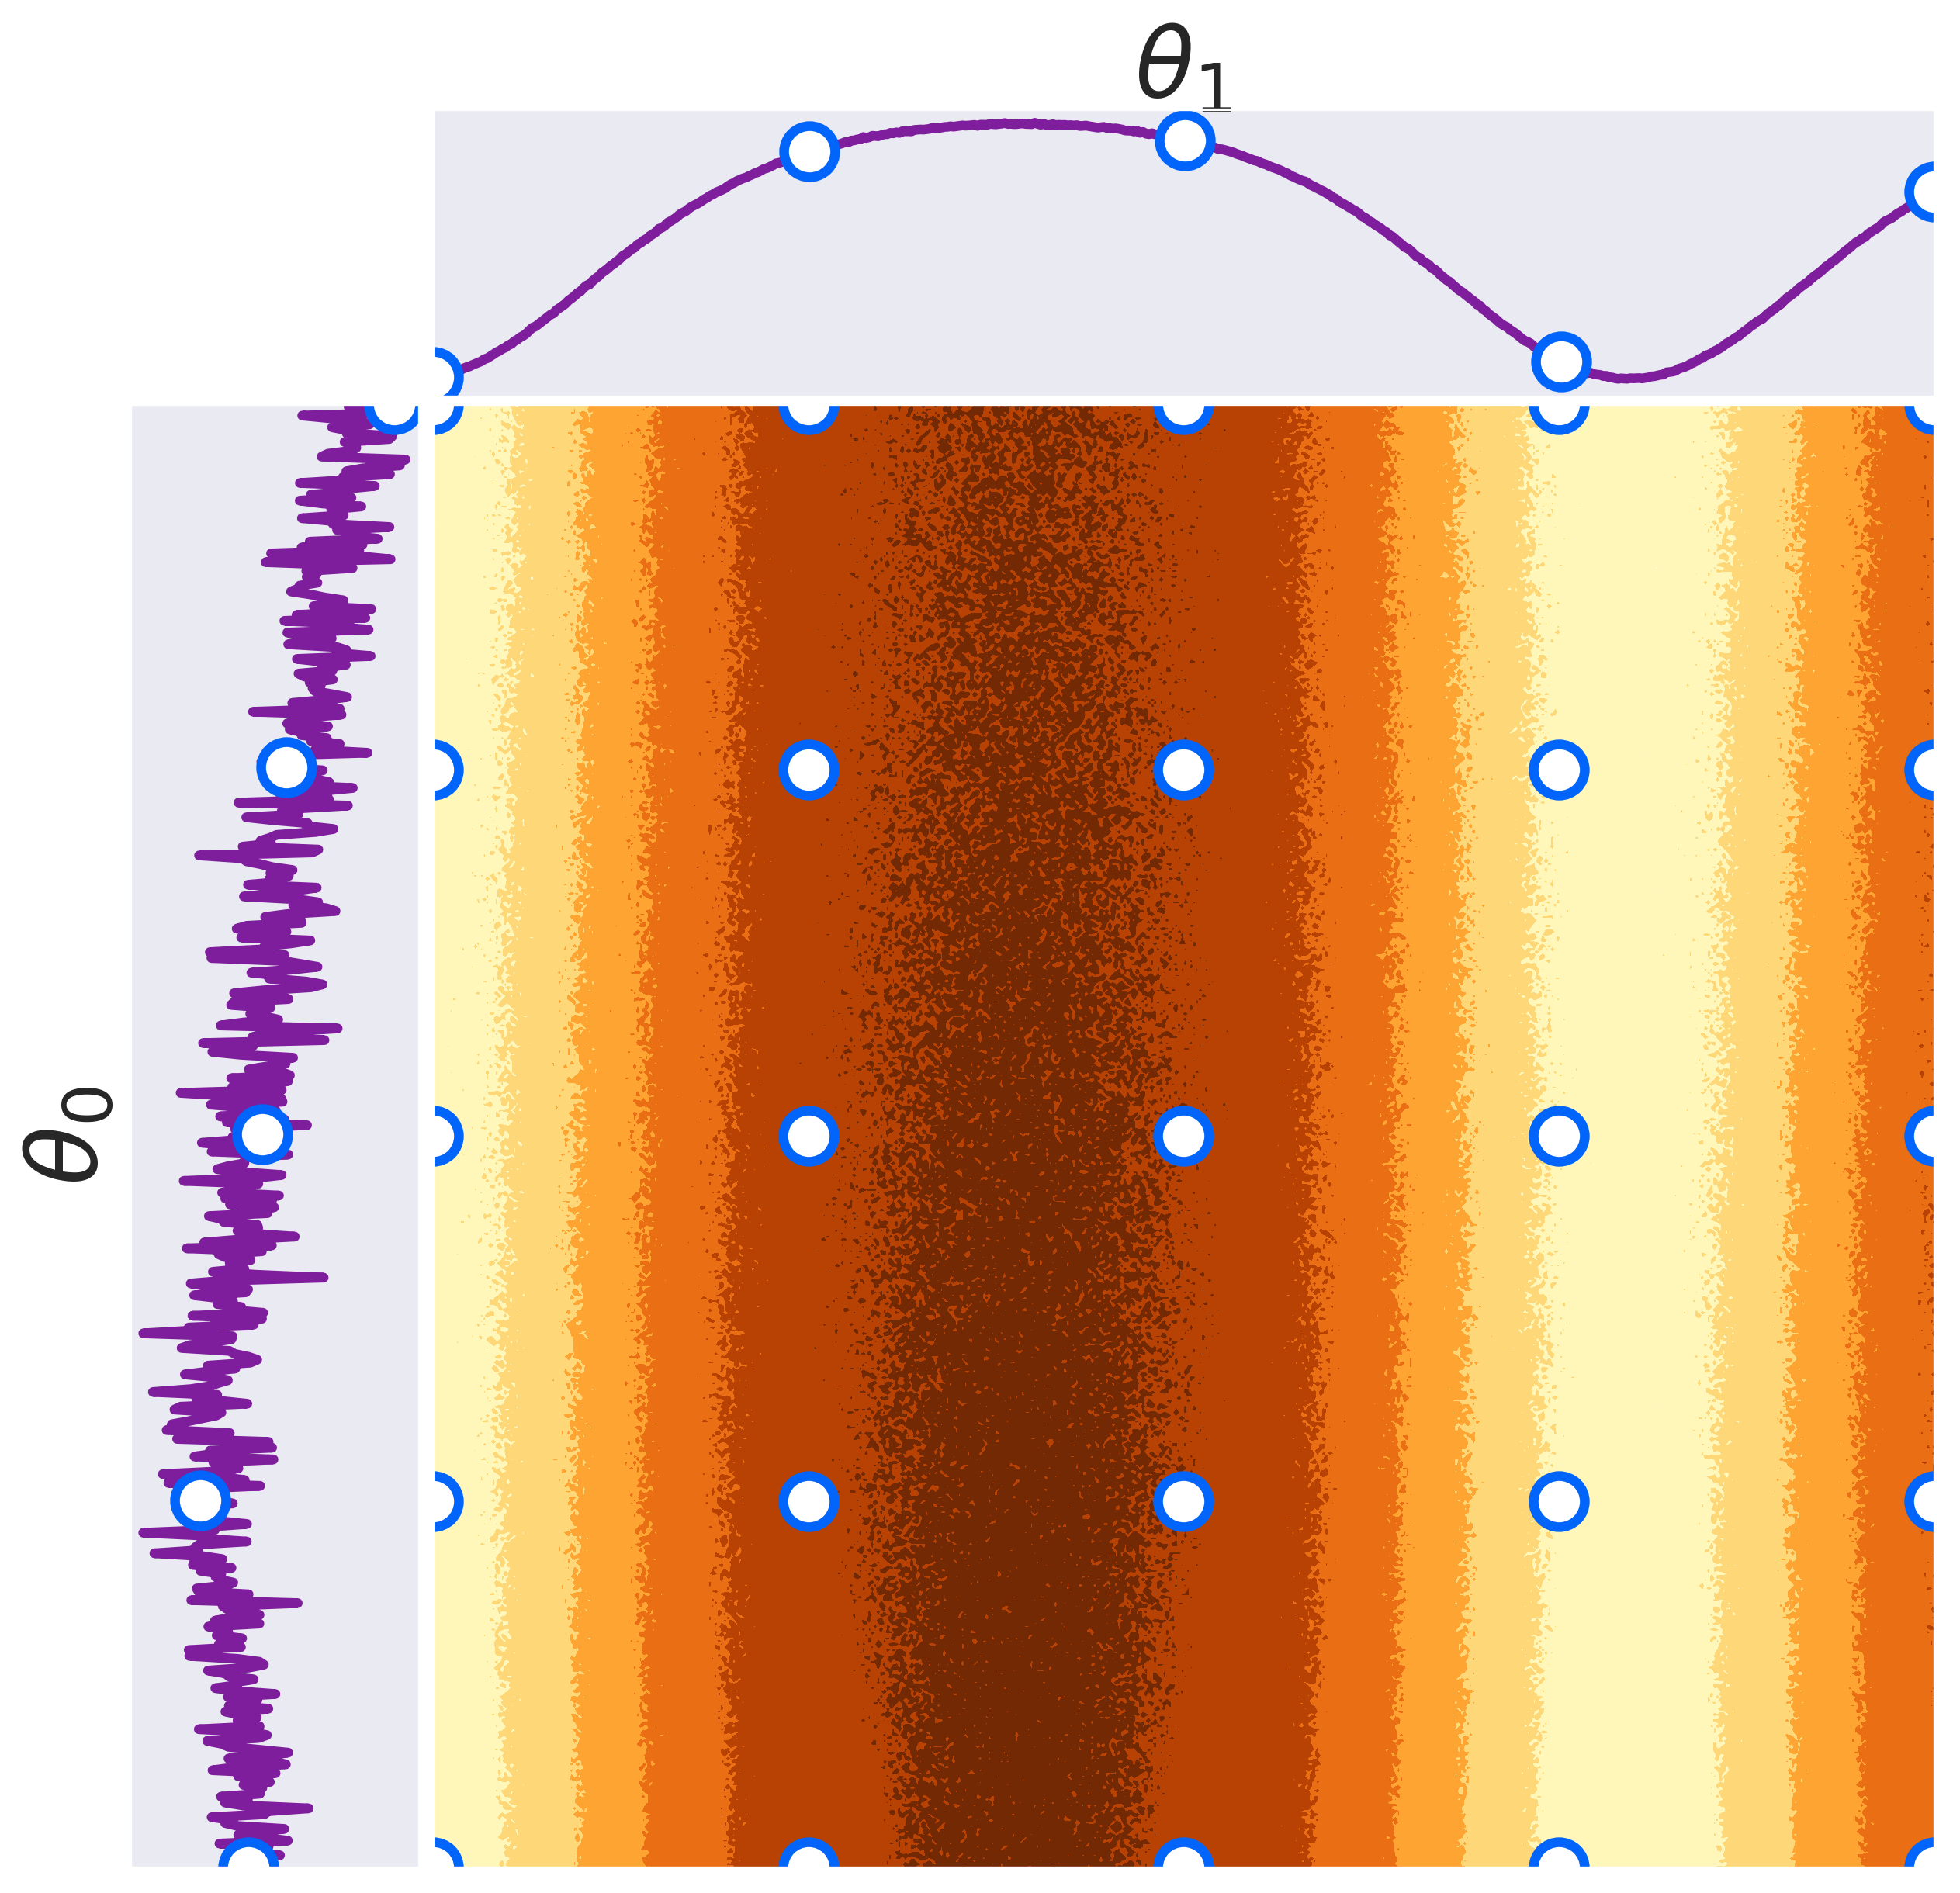
\includegraphics[width=0.28\textwidth]{plots/gs-vs-rs/gs}
\end{center}

\begin{block}{Pros and Cons}

\only<1-2>{\hands What are potential pros and cons of grid search?}
\pause

\begin{columns}
\column{0.4\textwidth}
Pros:
\begin{itemize}
  \item easy to implement
  \item easy to parallelize 
\end{itemize}

\column{0.6\textwidth}
Cons:
\begin{itemize}
  \item how to discretize space $\pcs$?
  \item does not scale with $\#$hyper-parameters
  \item inefficient if not all hyper-parameters are important
\end{itemize}


\end{columns}

\end{block}

\end{frame}
%-----------------------------------------------------------------------
%-----------------------------------------------------------------------
\begin{frame}[c,fragile]{Random Search \litw{Bergstra et al. '12}}

\begin{center}
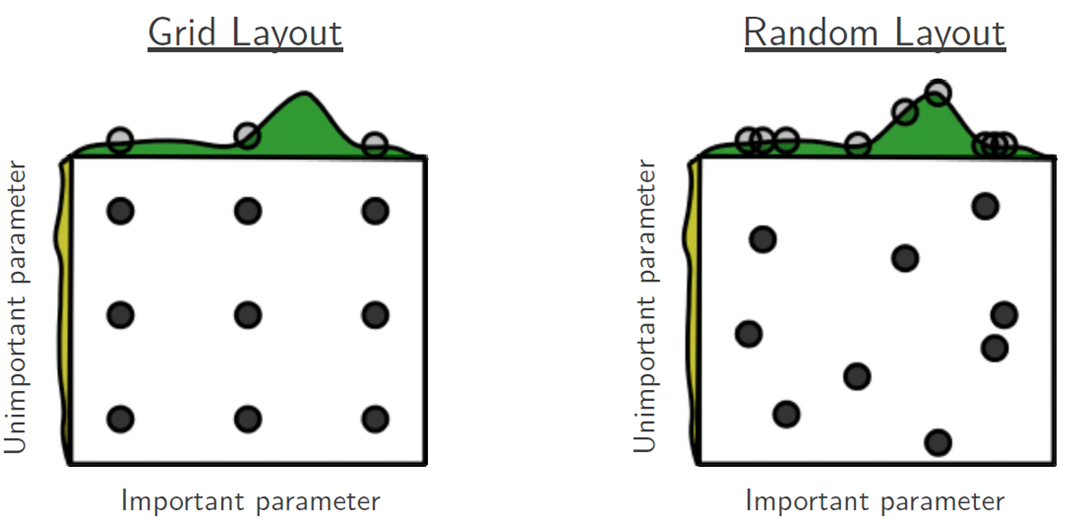
\includegraphics[width=0.28\textwidth]{plots/random_search}%
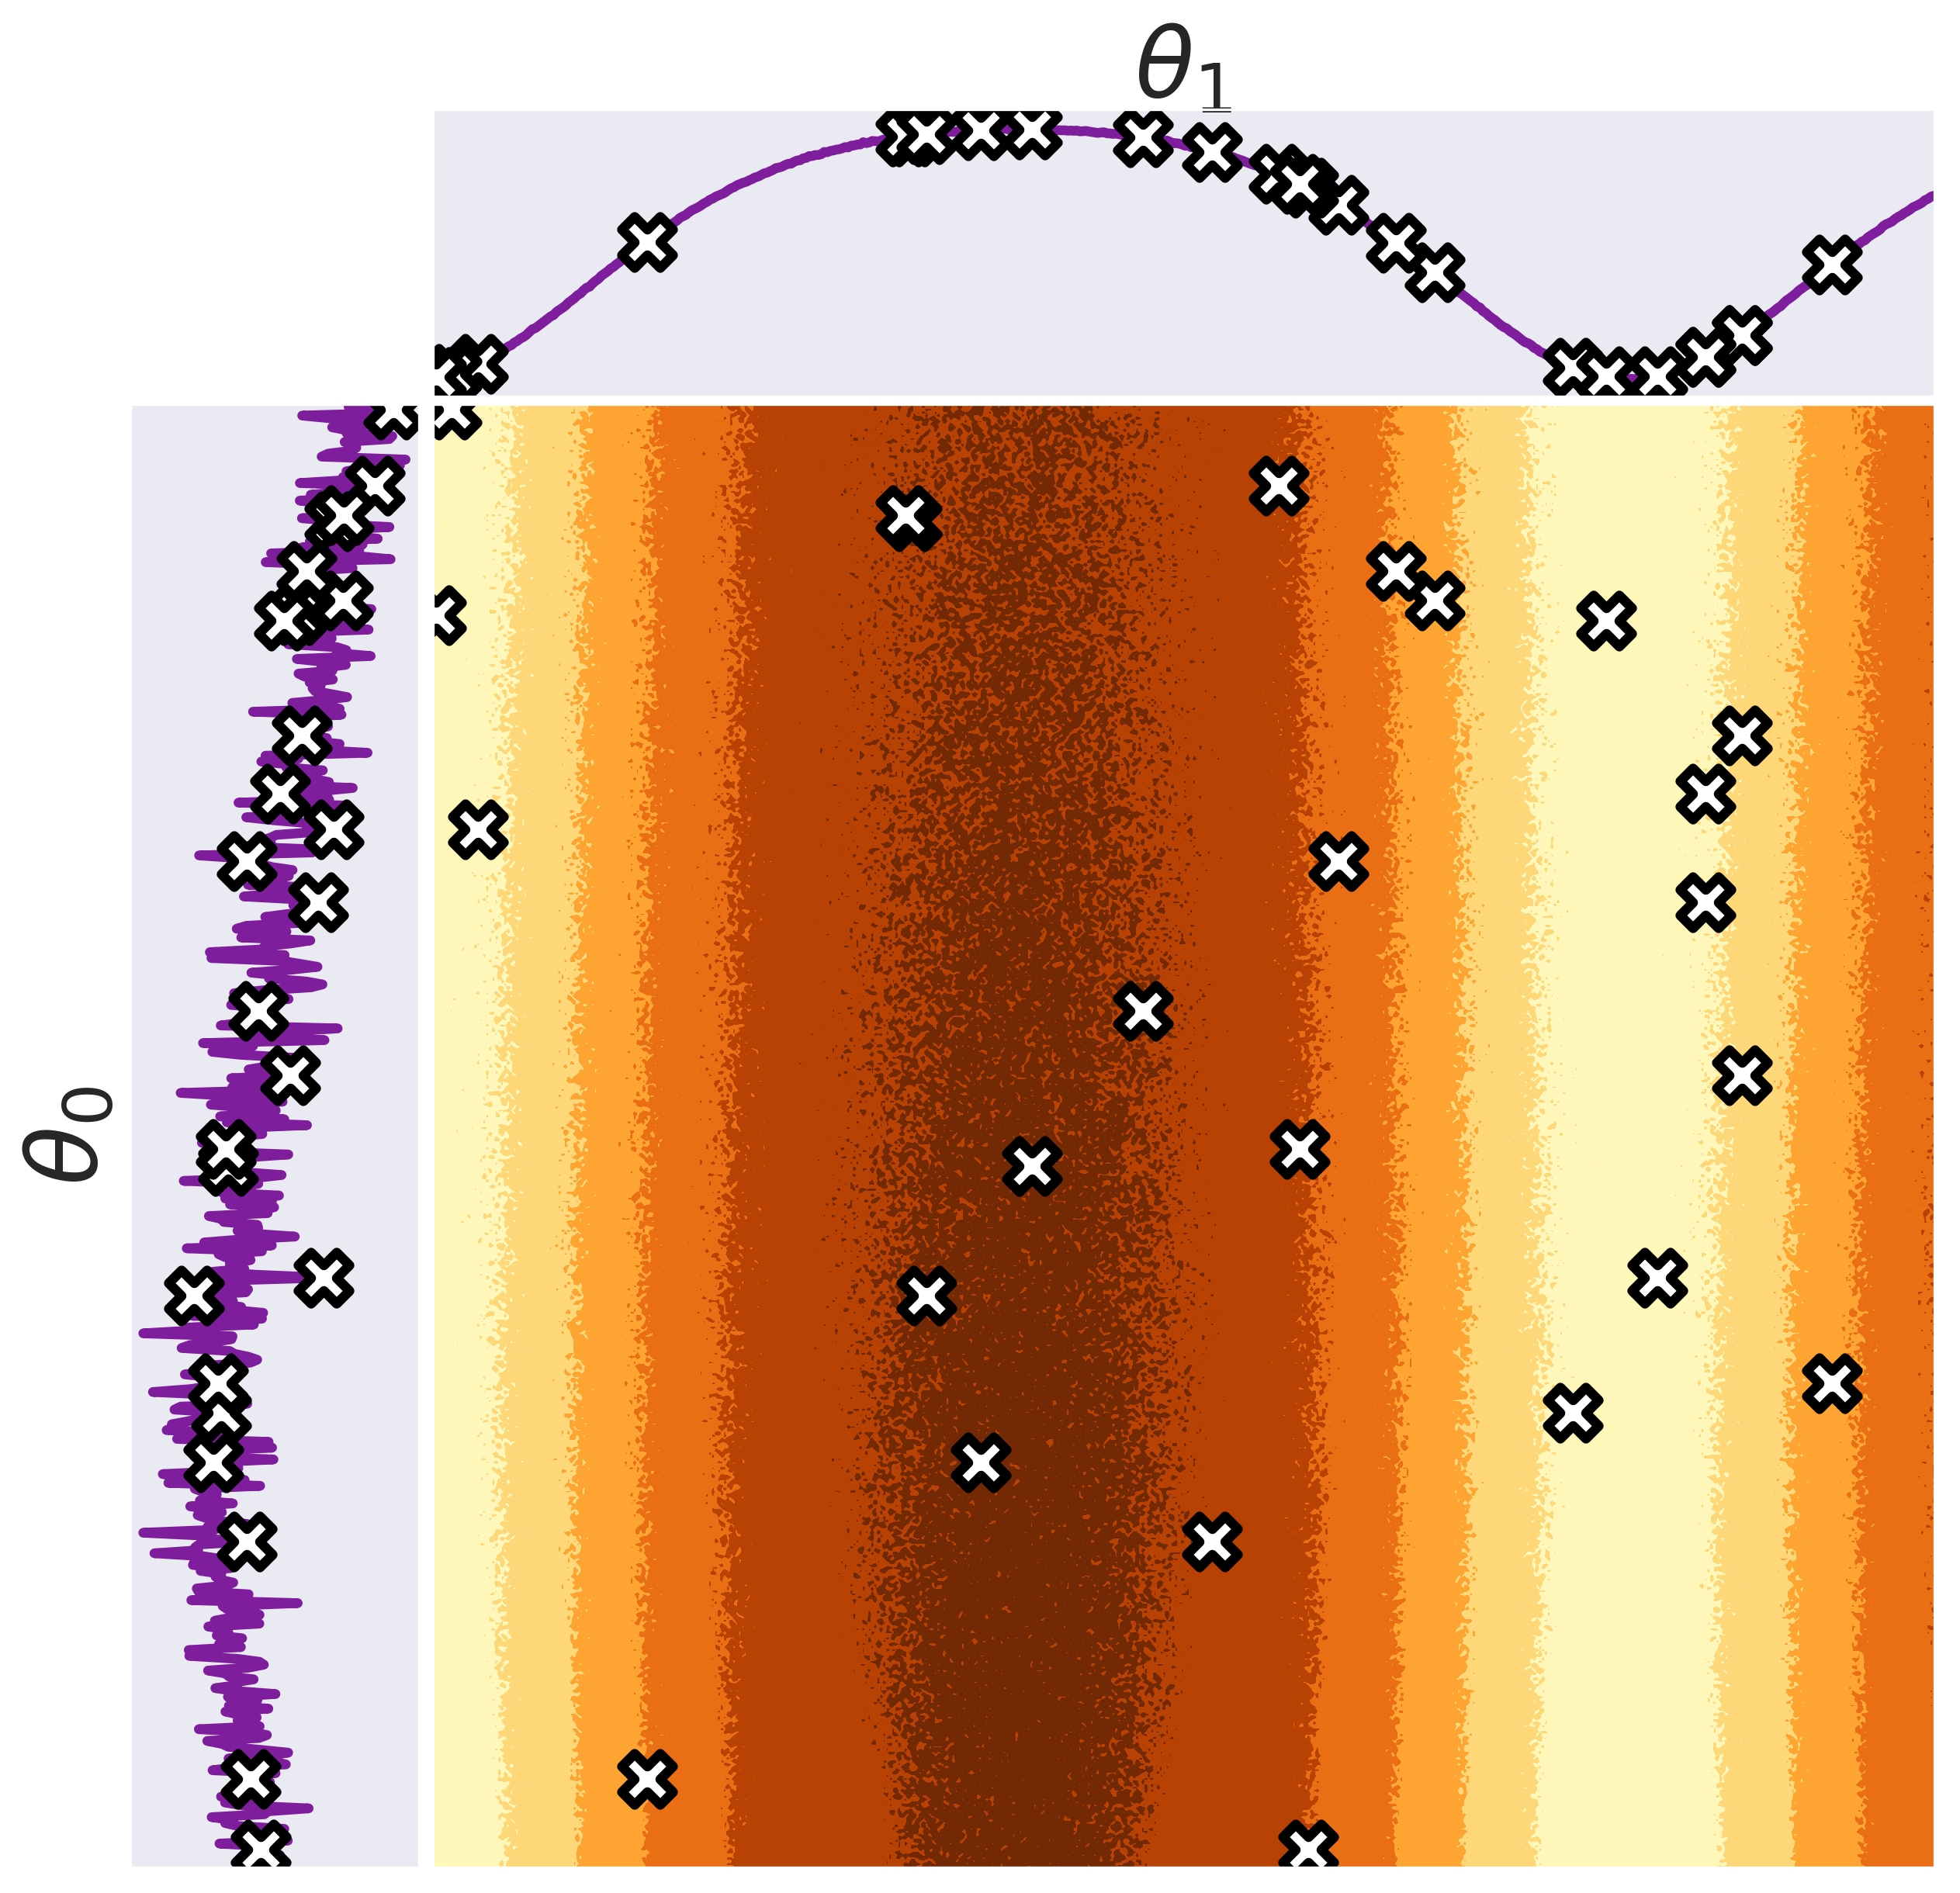
\includegraphics[width=0.28\textwidth]{plots/gs-vs-rs/rs}
\end{center}

\begin{block}{Pros and Cons}

\only<1-2>{\hands What are potential pros and cons of random search?}
\pause

\begin{columns}
\column{0.4\textwidth}
Pros:
\begin{itemize}
  \item even easier to implement
  \item easy to parallelize 
  \item more evaluations along each parameter
\end{itemize}

\column{0.6\textwidth}
Cons:
\begin{itemize}
  \item does not scale with $\#$hyper-parameters
  \item purely explorative
\end{itemize}


\end{columns}

\end{block}

\end{frame}
%-----------------------------------------------------------------------

%-----------------------------------------------------------------------
\begin{frame}[c,fragile]{Bayesian Optimization \litw{J. Mockus 1977}}

\begin{columns}

\column{0.4\textwidth}

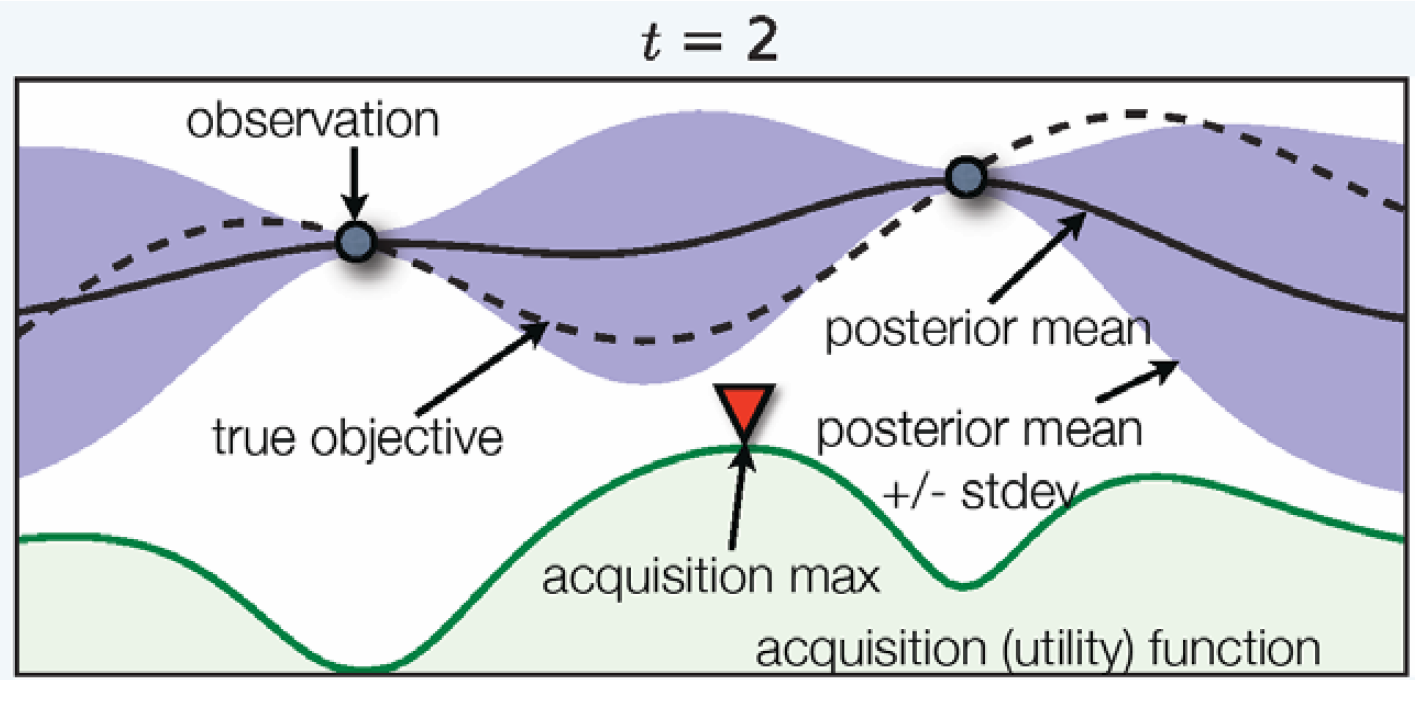
\includegraphics[width=\textwidth]{images/my_lecture12/bo_pic1.png}\\
\pause
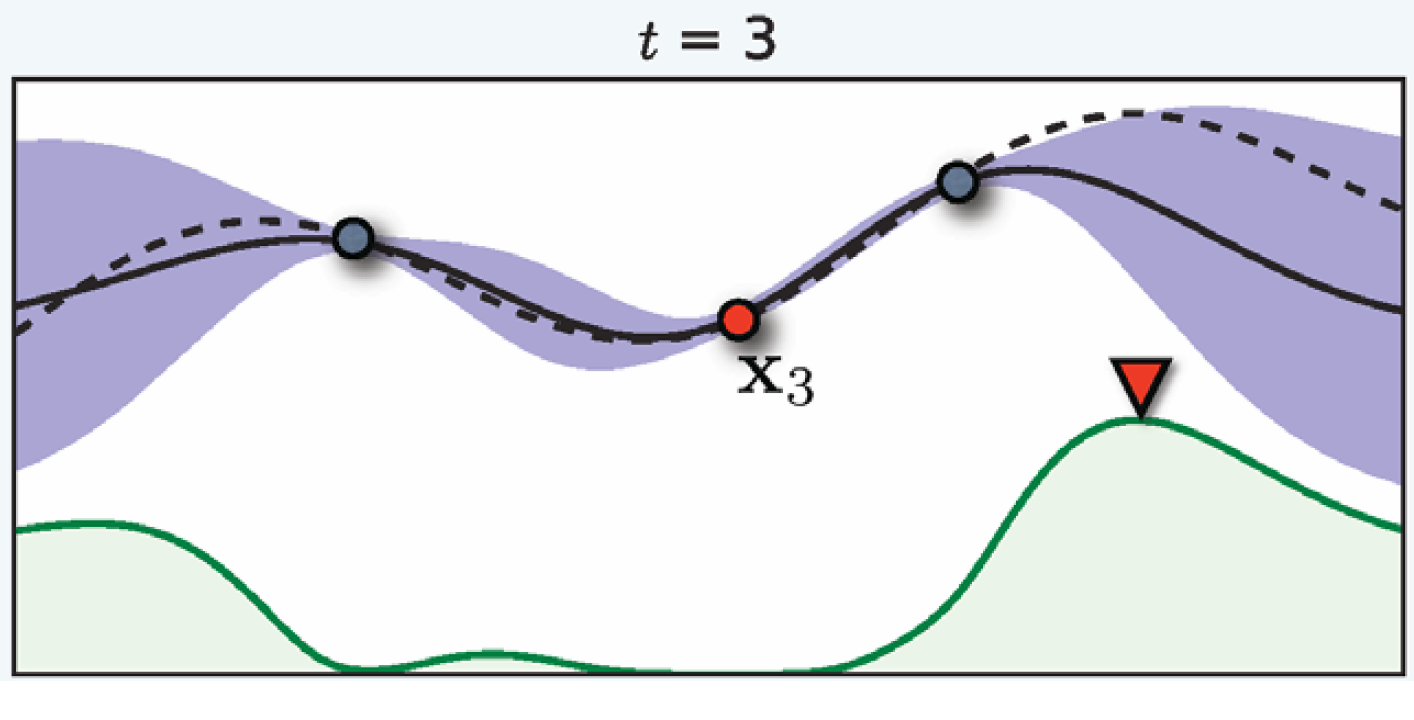
\includegraphics[width=\textwidth]{images/my_lecture12/bo_pic2.png}\\
\pause
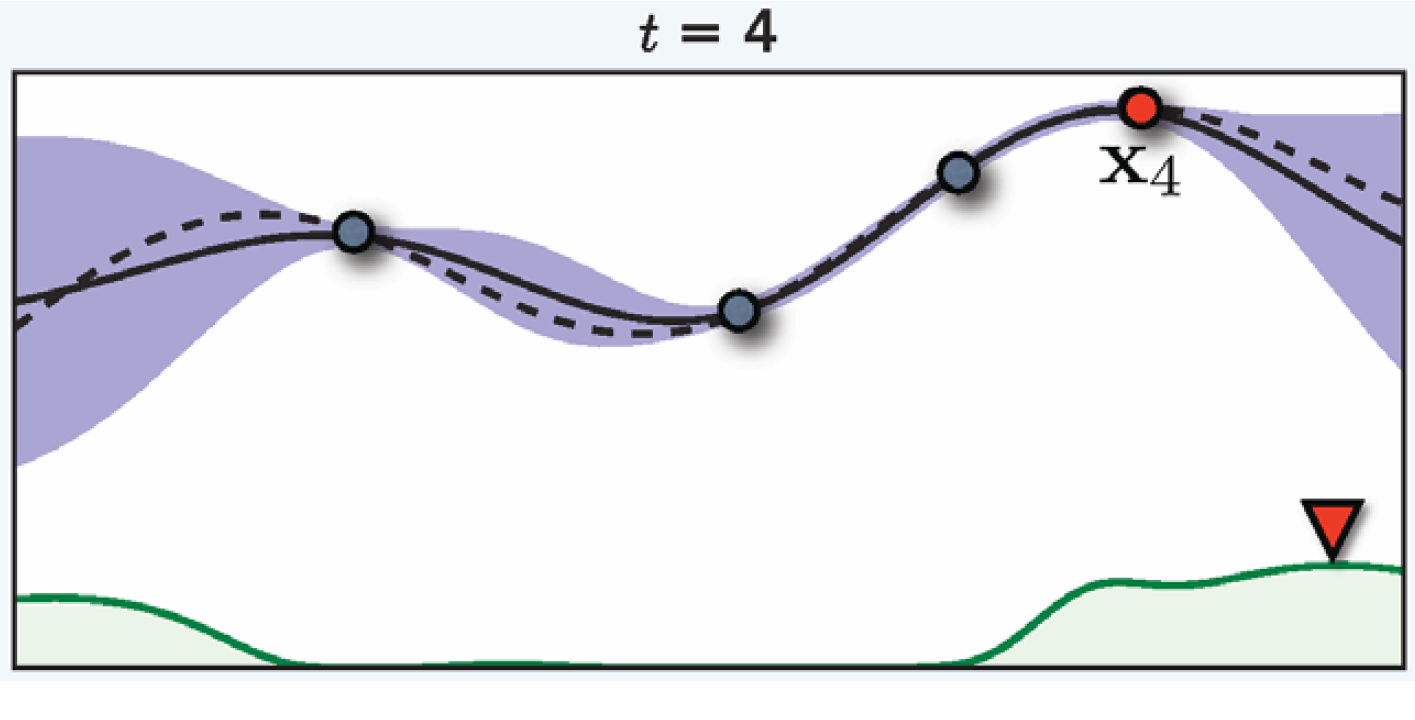
\includegraphics[width=\textwidth]{images/my_lecture12/bo_pic3.png}
\pause

\column{0.55\textwidth}
General Approach:
\begin{enumerate}
  \item Fit model on collected observations $\langle{}\conf, f(\conf)\rangle{}$
  \pause
  \item use acquisition function $a$ to trade off exploration and exploitation
  \pause
  \item maximize acquisition function: $x^* \in \argmin a(x)$
  \pause
  \item obtain new observation at $x^*$
\end{enumerate}

\pause
Moving pieces:
\begin{itemize}
  	\item Which \alert{model family} to use 
	\item How to use the model to guide optimization
	\begin{itemize}
		\item Determined by $a(x)$\\
		(Which data point should I \emph{acquire} next?) 
	\end{itemize}
\end{itemize}

\end{columns}

\end{frame}
%-----------------------------------------------------------------------

%-----------------------------------------------------------------------
\begin{frame}[c,fragile]{Bayesian Optimization}

\begin{block}{Pros and Cons}

Pros:
\begin{itemize}
  \item sample efficient
  \item can be applied to many black-box functions with expensive function evaluations (not only HPO)
\end{itemize}

Cons:
\begin{itemize}
  \item overhead because of model training in each iteration
  \item hard to parallelize
  \item (requires good model (EPM))
\end{itemize}

\end{block}

\end{frame}
%-----------------------------------------------------------------------


%%%%%%%%%%%%%%%%%%%%%%%%%%%%%%%%%%%%%%%%%%%%%%%%%%%%%%%%%%%%%%%%%%%%%%%%%
\begin{frame}[c,fragile]{The Role of the Acquisition Function}
\begin{itemize}
  \item Given: a model $\hat{f}:\confs \rightarrow \mathds{R}$ that predicts the quality $\mu(\conf)$ for each configuration $\conf$ and its standard deviation $\sigma(\conf)$ ($\leadsto$ uncertainty)
  \myit{
  	\item Assume w.l.o.g. that we want to \emph{maximize} $f$
  } 
  \medskip
  \mypause
  \item Which configuration should we select next? Need to trade off: 
  \begin{itemize}
    \item \alert{Exploitation}\\(sampling where the predicted mean $\mu(\conf)$ is high)
    \item \alert{Exploration}\\(sampling where we're uncertain about f; i.e., $\sigma(\conf)$ is high)
  \end{itemize}
  \medskip
  \mypause
  \item Various acquisition functions achieve this trade-off
\end{itemize}

\end{frame}
%%%%%%%%%%%%%%%%%%%%%%%%%%%%%%%%%%%%%%%%%%%%%%%%%%%%%%%%%%%%%%%%%%%%%%%%%


%%%%%%%%%%%%%%%%%%%%%%%%%%%%%%%%%%%%%%%%%%%%%%%%%%%%%%%%%%%%%%%%%%%%%%%%%
\begin{frame}[c,fragile]{Probability of Improvement}
\begin{itemize}
\vspace*{-0.2cm}
  \item Let $f(\theta^+)$ denote the best (here: max) function value known so far.
\vspace*{-0.2cm}  
  \begin{eqnarray}
\nonumber{}  PI(\conf) & = & P(f(\conf) \ge f(\theta^+))) = \Phi \left( \frac{\mu(\theta) - f(\theta^+)}{\sigma(\theta)} \right)
  \end{eqnarray}
  \item Here, $\Phi$ is the cumulative distribution function of the standard normal distribution. (There are $\mathcal{O}(1)$ lookup tables for this.)
\end{itemize}
\centering
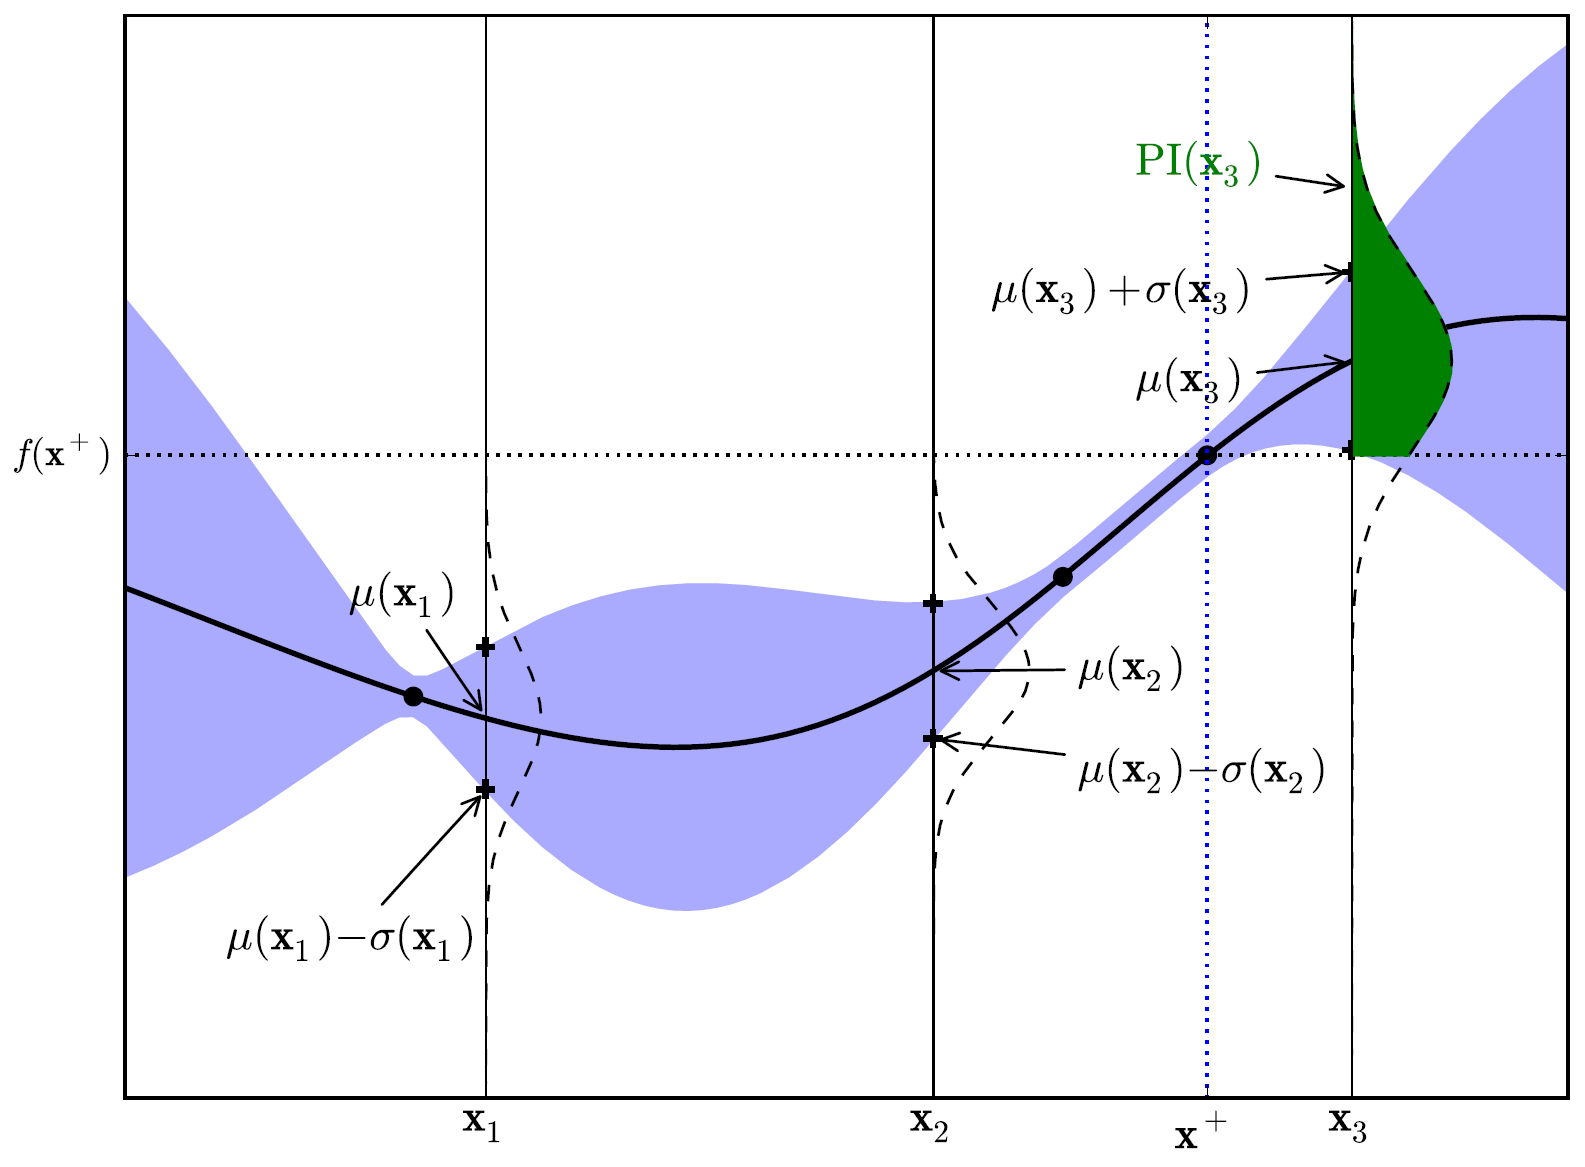
\includegraphics[width=0.55\textwidth]{plots/Acquisition-PI.png} 

\end{frame}
%%%%%%%%%%%%%%%%%%%%%%%%%%%%%%%%%%%%%%%%%%%%%%%%%%%%%%%%%%%%%%%%%%%%%%%%%

%%%%%%%%%%%%%%%%%%%%%%%%%%%%%%%%%%%%%%%%%%%%%%%%%%%%%%%%%%%%%%%%%%%%%%%%%
\begin{frame}[c,fragile]{Expected Improvement}

\begin{itemize}
\vspace*{-0.2cm}
  \item Like probability of improvement, but also takes into account the \alert{magnitude} of the improvement.
  \item Define the improvement at a point $\conf$ as:\\
\vspace*{-0.2cm}
  \begin{equation}
  \nonumber{}I(\conf) = \max (f(\conf) - f(\conf^+), 0)
  \end{equation}
  \mypause
\vspace*{-0.4cm}  
  \item Then, we can compute the expectation of this improvement across the predictive distribution
  \begin{eqnarray}
\nonumber{} \mathds{E}[I(x)] = \int_{-\infty}^{\infty} \max (f(\conf) - f(\conf^+), 0) \cdot \norm( f(\conf) ; \mu(\conf), \sigma^2(\conf) )  df(\conf) 
  \end{eqnarray}
  \mypause
\vspace*{-0.2cm}
  \item This turns out to have a closed form solution:
  \small
  \begin{eqnarray}
\nonumber{} \mathds{E}[I(x)] = (\mu(\conf) - f^+) \Phi\left( \frac{\mu(\conf) - f(\conf^+)}{\sigma(\conf)} \right)  + \sigma(\conf) \phi \left( \frac{\mu(\conf) - f(\conf^+)}{\sigma(\conf)} \right)
  \end{eqnarray}
\end{itemize}

\end{frame}
%%%%%%%%%%%%%%%%%%%%%%%%%%%%%%%%%%%%%%%%%%%%%%%%%%%%%%%%%%%%%%%%%%%%%%%%%

%%%%%%%%%%%%%%%%%%%%%%%%%%%%%%%%%%%%%%%%%%%%%%%%%%%%%%%%%%%%%%%%%%%%%%%%%
\begin{frame}[c,fragile]{Upper Confidence Bound}
\begin{itemize}
\vspace*{-0.2cm}
  \item UCB$(\conf) = \mu(\conf) + \kappa\sigma(\conf)$, with exploration parameter $\kappa$
\end{itemize}
\vspace*{-0.2cm}  
\centering
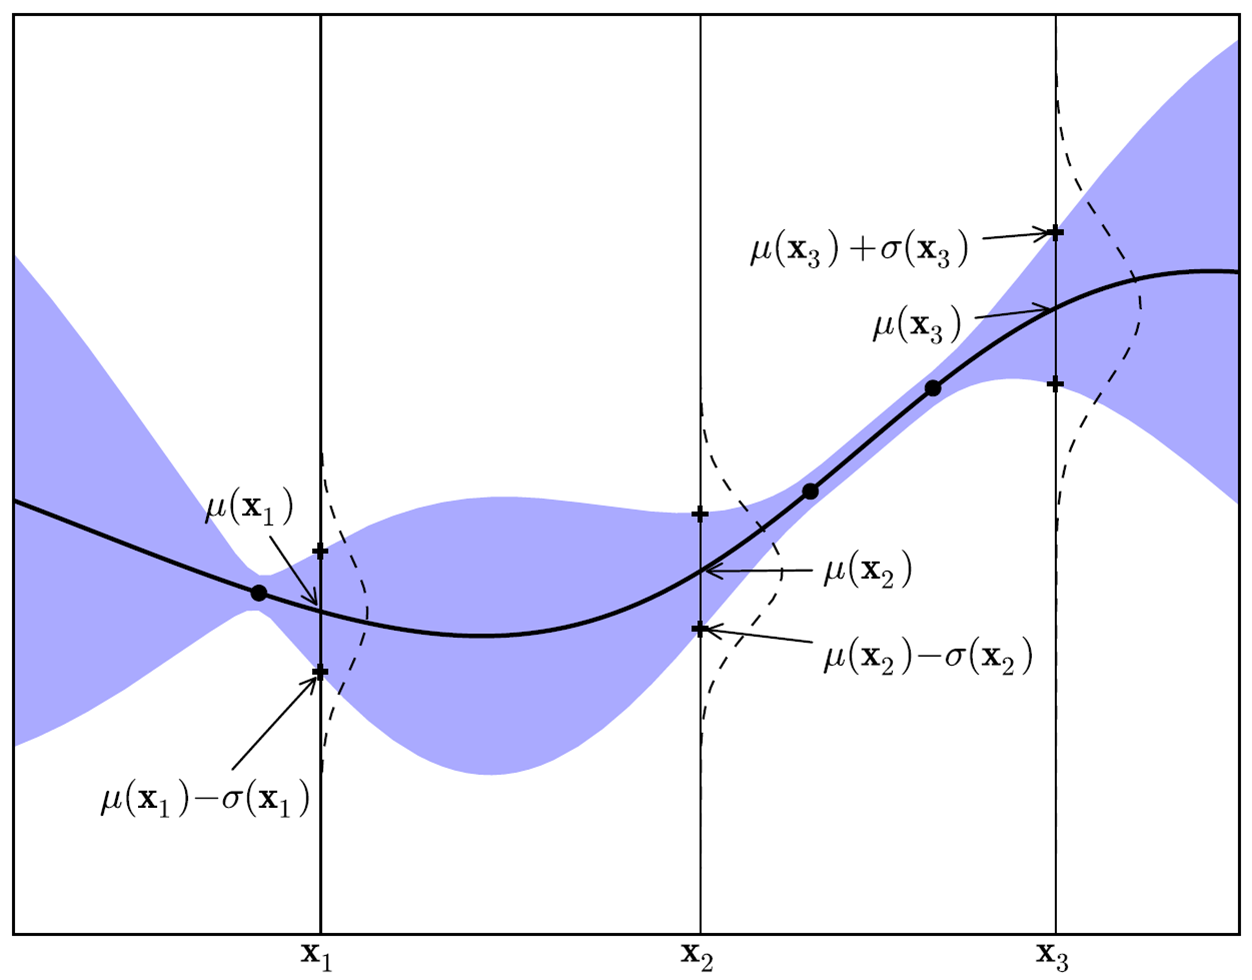
\includegraphics[width=0.55\textwidth]{plots/Acquisition-UCB.png} 
\vspace*{0.2cm}  
\begin{itemize}
\item Which point would we pick next with UCB and $\kappa = 1$? \hands
\mypause
 \item GP-UCB$(\conf) = \mu(\conf) + \sqrt{\beta_t} \sigma(\conf)$, with $\beta_t$ \alert{increasing} over time
\end{itemize}

\end{frame}
%%%%%%%%%%%%%%%%%%%%%%%%%%%%%%%%%%%%%%%%%%%%%%%%%%%%%%%%%%%%%%%%%%%%%%%%%

%%%%%%%%%%%%%%%%%%%%%%%%%%%%%%%%%%%%%%%%%%%%%%%%%%%%%%%%%%%%%%%%%%%%%%%%%
\begin{frame}[c,fragile]{Empirical Performance Model}

Required features

\begin{itemize}
  \item Mandatory:
  \begin{itemize}
    \item Regression model
	\item Uncertainty estimates
  \end{itemize}
  \pause
  \item Preferable:
  \begin{itemize}
    \item accurate predictions
    \item cheap-to-train
    \item scales with the complexity of the data\\ (number of features and observations)
    \item can handle different types of features\\ (categorical and continuous)
  \end{itemize}
\end{itemize}

\pause
Our choice: Random Forests

\end{frame}
%%%%%%%%%%%%%%%%%%%%%%%%%%%%%%%%%%%%%%%%%%%%%%%%%%%%%%%%%%%%%%%%%%%%%%%%%

%%%%%%%%%%%%%%%%%%%%%%%%%%%%%%%%%%%%%%%%%%%%%%%%%%%%%%%%%%%%%%%%%%%%%%%%%
\begin{frame}[c,fragile]{Recap Random Forests}


\centering
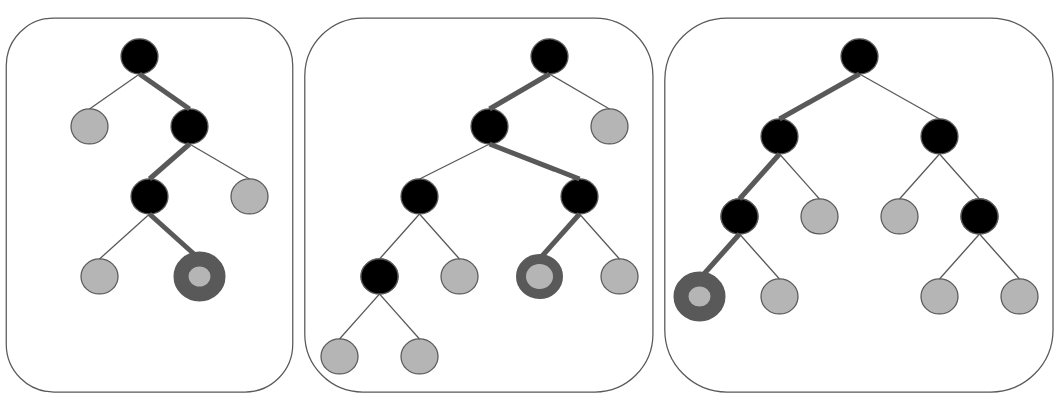
\includegraphics[width=0.55\textwidth]{images/random_forest_pic}

\begin{itemize}
  \item Train:
  \begin{itemize}
    \item $n$ decision (or regression) trees (potentially with pruning)
    \item subsampled training data for each tree (with bootstrapping)
    \item subsampled feature set for each split
  \end{itemize}
  \item Predict
  \begin{itemize}
    \item Obtain prediction of each tree
    \item Aggregate predictions (voting, average, \ldots)
    \pause
    \item Uncertainty predictions: average across tree predictions 
  \end{itemize}
\end{itemize}


\end{frame}
%%%%%%%%%%%%%%%%%%%%%%%%%%%%%%%%%%%%%%%%%%%%%%%%%%%%%%%%%%%%%%%%%%%%%%%%%
%%%%%%%%%%%%%%%%%%%%%%%%%%%%%%%%%%%%%%%%%%%%%%%%%%%%%%%%%%%%%%%%%%%%%%%%%
\begin{frame}[c,fragile]{Advantages and Disadvantages of Random Forests}


\begin{columns}
\column{0.5\textwidth}
Pros:
\begin{itemize}
  \item Cheap to train
  \item Scale well with the number of observations
  \begin{itemize}
    \item Worst-case complexity for $T$ tress with $n$ data points of dimensionality $p$: $\mathcal O(T\cdot p \cdot n^2 \log{n})$
  \end{itemize}
  \item training can be parallelized
  \item Can handle continuous and categorical features
  \begin{itemize}
    \item most RF implementations can handle only continuous features
  \end{itemize}
\end{itemize}

\column{0.5\textwidth}
Cons:
\begin{itemize}
  \item Poor uncertainty estimates
  \item No extrapolation
  \begin{itemize}
    \item last seen value for extrapolation (constant)
  \end{itemize}
\end{itemize}

\end{columns}

\end{frame}
%%%%%%%%%%%%%%%%%%%%%%%%%%%%%%%%%%%%%%%%%%%%%%%%%%%%%%%%%%%%%%%%%%%%%%%%%
%----------------------------------------------------------------------
{\setbeamertemplate{logo}{}
\begin{frame}[c]{What are Empirical Performance Models?}

\begin{block}{Definition: (Simplified) Empirical Performance Models (EPMs)}
Empirical performance models map
\begin{itemize} 
  \item parameter configuration $\conf \in \pcs$ of an algorithm 
  \item to the cost $m(\conf)$ of $\conf$ : 
\end{itemize}


\begin{equation}
\surro: \pcs \to \perf \nonumber
\end{equation}
\end{block}

\pause

\begin{block}{Examples of Cost Metrics}
\begin{itemize}
  \item runtime
  \item success probability of an algorithm
  \item solution quality an optimization algorithm achieves in a fixed time
  \item error of machine learning algorithm
\end{itemize}
\end{block}

\end{frame}}
%-----------------------------------------------------------------------
%----------------------------------------------------------------------
\begin{frame}[c]{Configuration Space}

\begin{block}{Types of Parameters}
  \begin{itemize}
    \item continuous parameter: value between $[l,u]$
    \begin{itemize}
      \item e.$\,$g., restart probability $wp \in [0,1]$ 
    \end{itemize}
    \pause
    \item integer parameter: integer value between $[l,u]$
    \begin{itemize}
      \item e.$\,$g., maximal number of splits in a decision tree in $[16,1024]$
    \end{itemize}
    \pause
    \item ordinal parameter: sorted list of values $\langle v_1, v_2, \ldots, v_j \rangle$
    \begin{itemize}
      \item distance between values is unknown
      \item e.$\,$g., vague quantities such as $\langle few, medium, many \rangle$
    \end{itemize}
    \pause
    \item categorical parameters: set of values $\{v_1, v_2, \ldots, v_j \}$
    \begin{itemize}
      \item no ordering
      \item e.$\,$g., choice of algorithm $\{$SVM, RF, DNN$\}$
    \end{itemize}
  \end{itemize}
\end{block}

\pause
\bigskip
\hands Other examples?

\end{frame}
%-----------------------------------------------------------------------
%----------------------------------------------------------------------
\begin{frame}[c]{Preprocessing Configuration}

\begin{block}{Convert $\conf$ for ML Model}
  \begin{itemize}
    \item continuous and integer parameter can be directly passed
    \begin{itemize}
      \item scaled to $[0,1]$
    \end{itemize}
    \pause
    \item categorical parameters should be encoded if necessary
    \begin{itemize}
      \item e.$\,$g., random forest can handle categorical parameter natively\\
      (Not all implementations are able to do it!) 
      \item use one-hot encoding if necessary:
      \begin{itemize}
        \item add new variable for each possible value $v_i$
        \item set one of these variable to one (depending on the configuration)
      \end{itemize}
    \end{itemize}
    \pause
    \item ordinal parameters can be converted to integers or also one-hot encoded
  \end{itemize}
\end{block}


\end{frame}
%-----------------------------------------------------------------------
%----------------------------------------------------------------------
\begin{frame}[c]{Preprocessing Configuration (cont'd)}

\begin{block}{Conditional Parameters}
  \begin{itemize}
    \item Configuration spaces often have a hierarchical structure
    \item e.$\,$g., parameter A is only active if heuristic H is used
    \pause
    \item[$\leadsto$] List of parameter values has missing entries because of inactive parameters
    \medskip
    \pause
    \item Fixes:
    \begin{itemize}
    	\item Impute missing data, e.$\,$g., by default setting
    	\item Mark these inactive parameters and let the EPM deal with it\\
    		  e.$\,$g., a random forest could only split on active parameters
    \end{itemize}
  \end{itemize}
\end{block}

\end{frame}
%-----------------------------------------------------------------------
%----------------------------------------------------------------------
{\setbeamertemplate{logo}{}
\begin{frame}[c]{Example: SVM}

\begin{block}{Configuration Space}
kernel categorical \{linear, rbf, polynomial, sigmoid\}\\
C float [0.001,1000.0]\\
shrinking categorical \{True,False\}\\
degree integer [1,5]\\
coef0 float [0.0, 10.0]\\
gamma categorical \{auto, value\}\\
gamma\_value float [0.0001,8]\\
\end{block}

\begin{block}{Conditional Constraints}
degree $\mid$ kernel in \{polynomial\}\\
coef0 $\mid$ kernel in \{polynomial, sigmoid\}\\
gamma\_value $\mid$ gamma in \{value\}
\end{block}

\end{frame}
}
%-----------------------------------------------------------------------
{\setbeamertemplate{logo}{}
\begin{frame}[c,fragile]{Important Design Dimensions in BO}

\only<1>{
\begin{block}{Transformation of y-values}
	\begin{minipage}{0.6\textwidth}
		\begin{figure}[H]
			\centering
			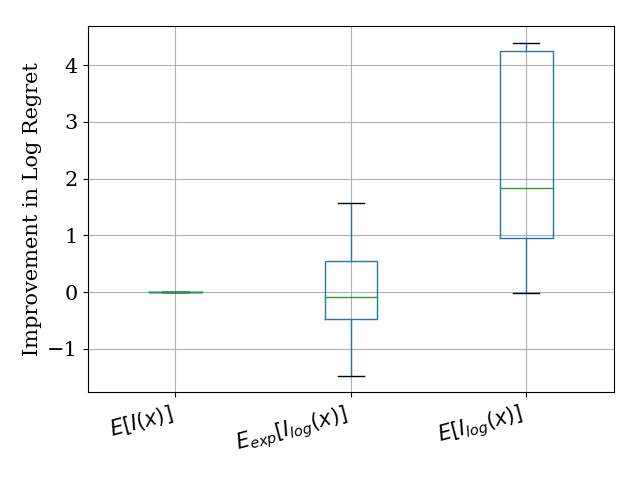
\includegraphics[height=.6\textheight]{plots/borf_boxplot_y}
		\end{figure}
	\end{minipage} \hfill
	\begin{minipage}{0.39\textwidth}
		\begin{itemize}
			\item log-transformed values to fit the model and the acquisition function improves performance
			\item less emphasize on large outlier values
			\item focus more on small improvements and less on exploration in unexplored spaces
		\end{itemize}
	\end{minipage}
\end{block}
}

\only<2>{
	\begin{block}{Interleaving Random Points}
		\begin{minipage}{0.6\textwidth}
			\begin{figure}[H]
				\centering
				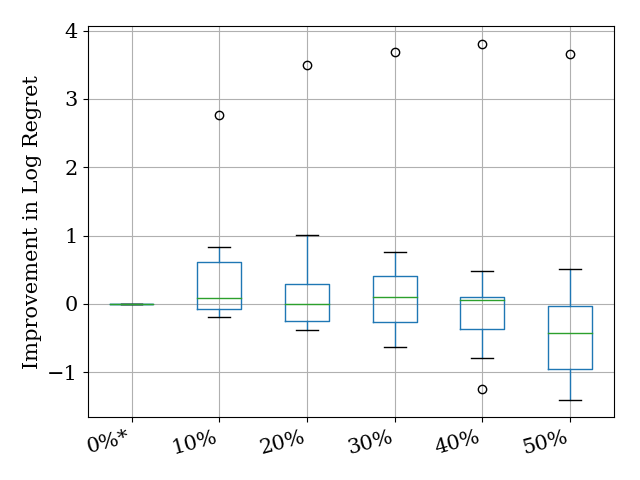
\includegraphics[height=.6\textheight]{plots/borf_boxplot_r}
			\end{figure}
		\end{minipage} \hfill
		\begin{minipage}{0.39\textwidth}
			\begin{itemize}
				\item RFs do not extrapolate well
				\item Interpolation between two observations with similar function values leads to
				constant uncertainty estimates
				\item BO with RFs can easily get stuck in local optima
				\item interleave randomly sampled points to escape local optima
			\end{itemize}
		\end{minipage}
	\end{block}
}

\only<3>{
	\begin{block}{Initial Design}
		\begin{minipage}{0.6\textwidth}
			\begin{figure}[H]
				\centering
				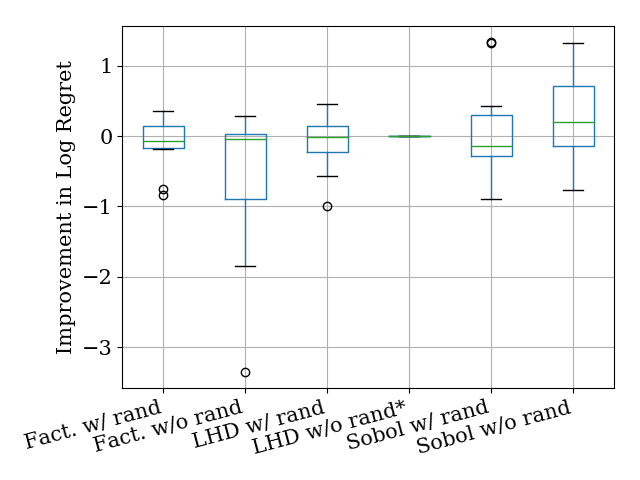
\includegraphics[height=.6\textheight]{plots/borf_boxplot_init}
			\end{figure}
		\end{minipage} \hfill
		\begin{minipage}{0.39\textwidth}
			\begin{itemize}
				\item Alternative to exploration via randomly sampled points
				\item explore the space before the actual BO takes place
				\item Pro: will improve the EPM in early iterations
				\item Con: will invest a considerable number of function evaluations without taking the already gathered knowledge into account
			\end{itemize}
		\end{minipage}
	\end{block}
}
\end{frame}
}
%-----------------------------------------------------------------------
\begin{frame}[c,fragile]{What if a single configuration is too expensive?}


\begin{itemize}
  \item Sometimes, even validating a single configuration needs a lot of time\\
  		e.$\,$g., single function evaluation takes hours or even days:
  \begin{itemize}
    \item ML on big data
    \item Training a deep neural network  
  \end{itemize}
  \pause
  \item Challenge: We cannot search for a configuration if we can afford very few function evaluations $< 10$
  \pause
  \item \hands What could we do?
  \pause
  \begin{itemize}
    \item Data subset selection
    \item Predict learning curves
  \end{itemize}
  \item[$\leadsto$] Going from black-box to grey-box optimization
\end{itemize}

\end{frame}
%-----------------------------------------------------------------------

%-----------------------------------------------------------------------
\begin{frame}[c,fragile]{Learning Curves}

\centering
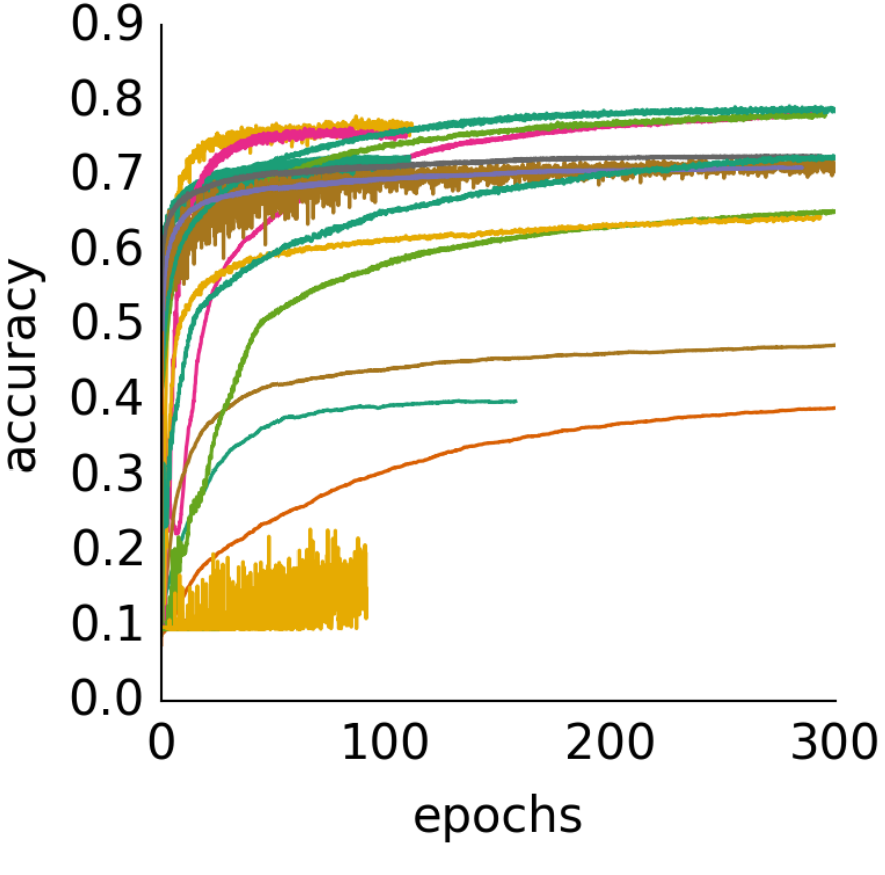
\includegraphics[width=0.5\textwidth]{images/learning_curves}

Exemplary learning curves of training deep neural networks\\
Many ML algorithms iteratively optimize a (loss) function

\end{frame}
%-----------------------------------------------------------------------

%-----------------------------------------------------------------------
\begin{frame}[c,fragile]{Learning Curve Predictions}

\centering
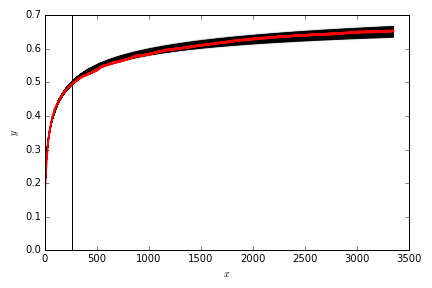
\includegraphics[width=0.6\textwidth]{images/learning_curve_single_pred}

\begin{enumerate}
  \item Observe learning curve for the first $n$ steps (here $n=250$)
  \pause
  \item Fit parametric model on partial learning curve to predict remaining learning curve
  \pause
  \item Which model to use? 
  \begin{itemize}
    \item Good model depends on shape of curve $\to$ e.$\,$g., depends on optimizer  
    \item[$\leadsto$] combination of several models
  \end{itemize}
  
\end{enumerate}

\end{frame}
%-----------------------------------------------------------------------

%-----------------------------------------------------------------------
\begin{frame}[c,fragile]{Learning Curves: Early Termination}

\centering
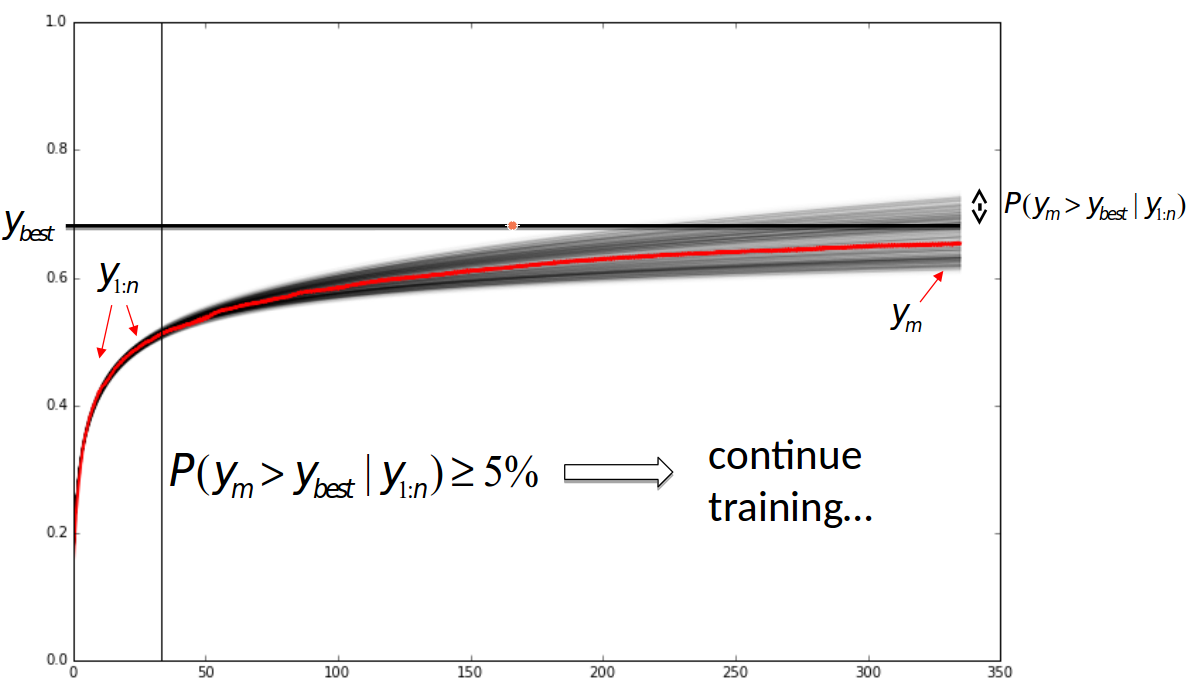
\includegraphics[width=\textwidth]{images/learning_curve_dec}

\end{frame}
%-----------------------------------------------------------------------
%-----------------------------------------------------------------------
\begin{frame}[c,fragile]{Learning Curves: Early Termination}

\centering
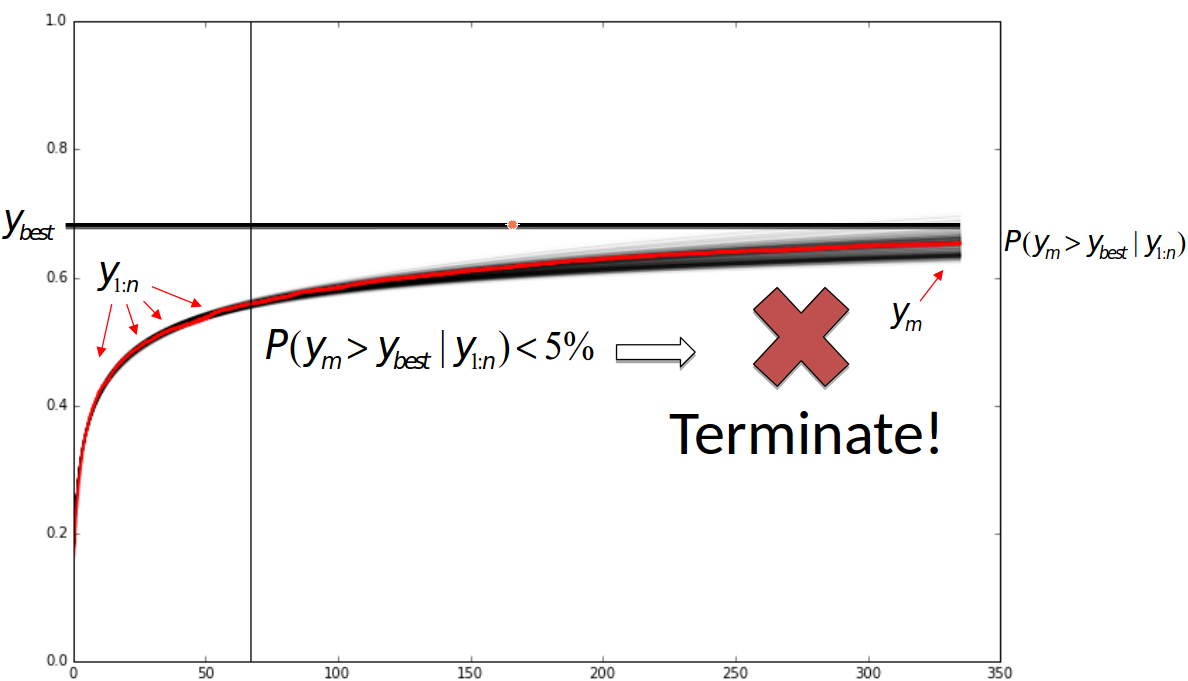
\includegraphics[width=\textwidth]{images/learning_curve_dec2}

\end{frame}
%-----------------------------------------------------------------------
%-----------------------------------------------------------------------
\begin{frame}[c,fragile]{Learning Curves: Early Termination}

\centering
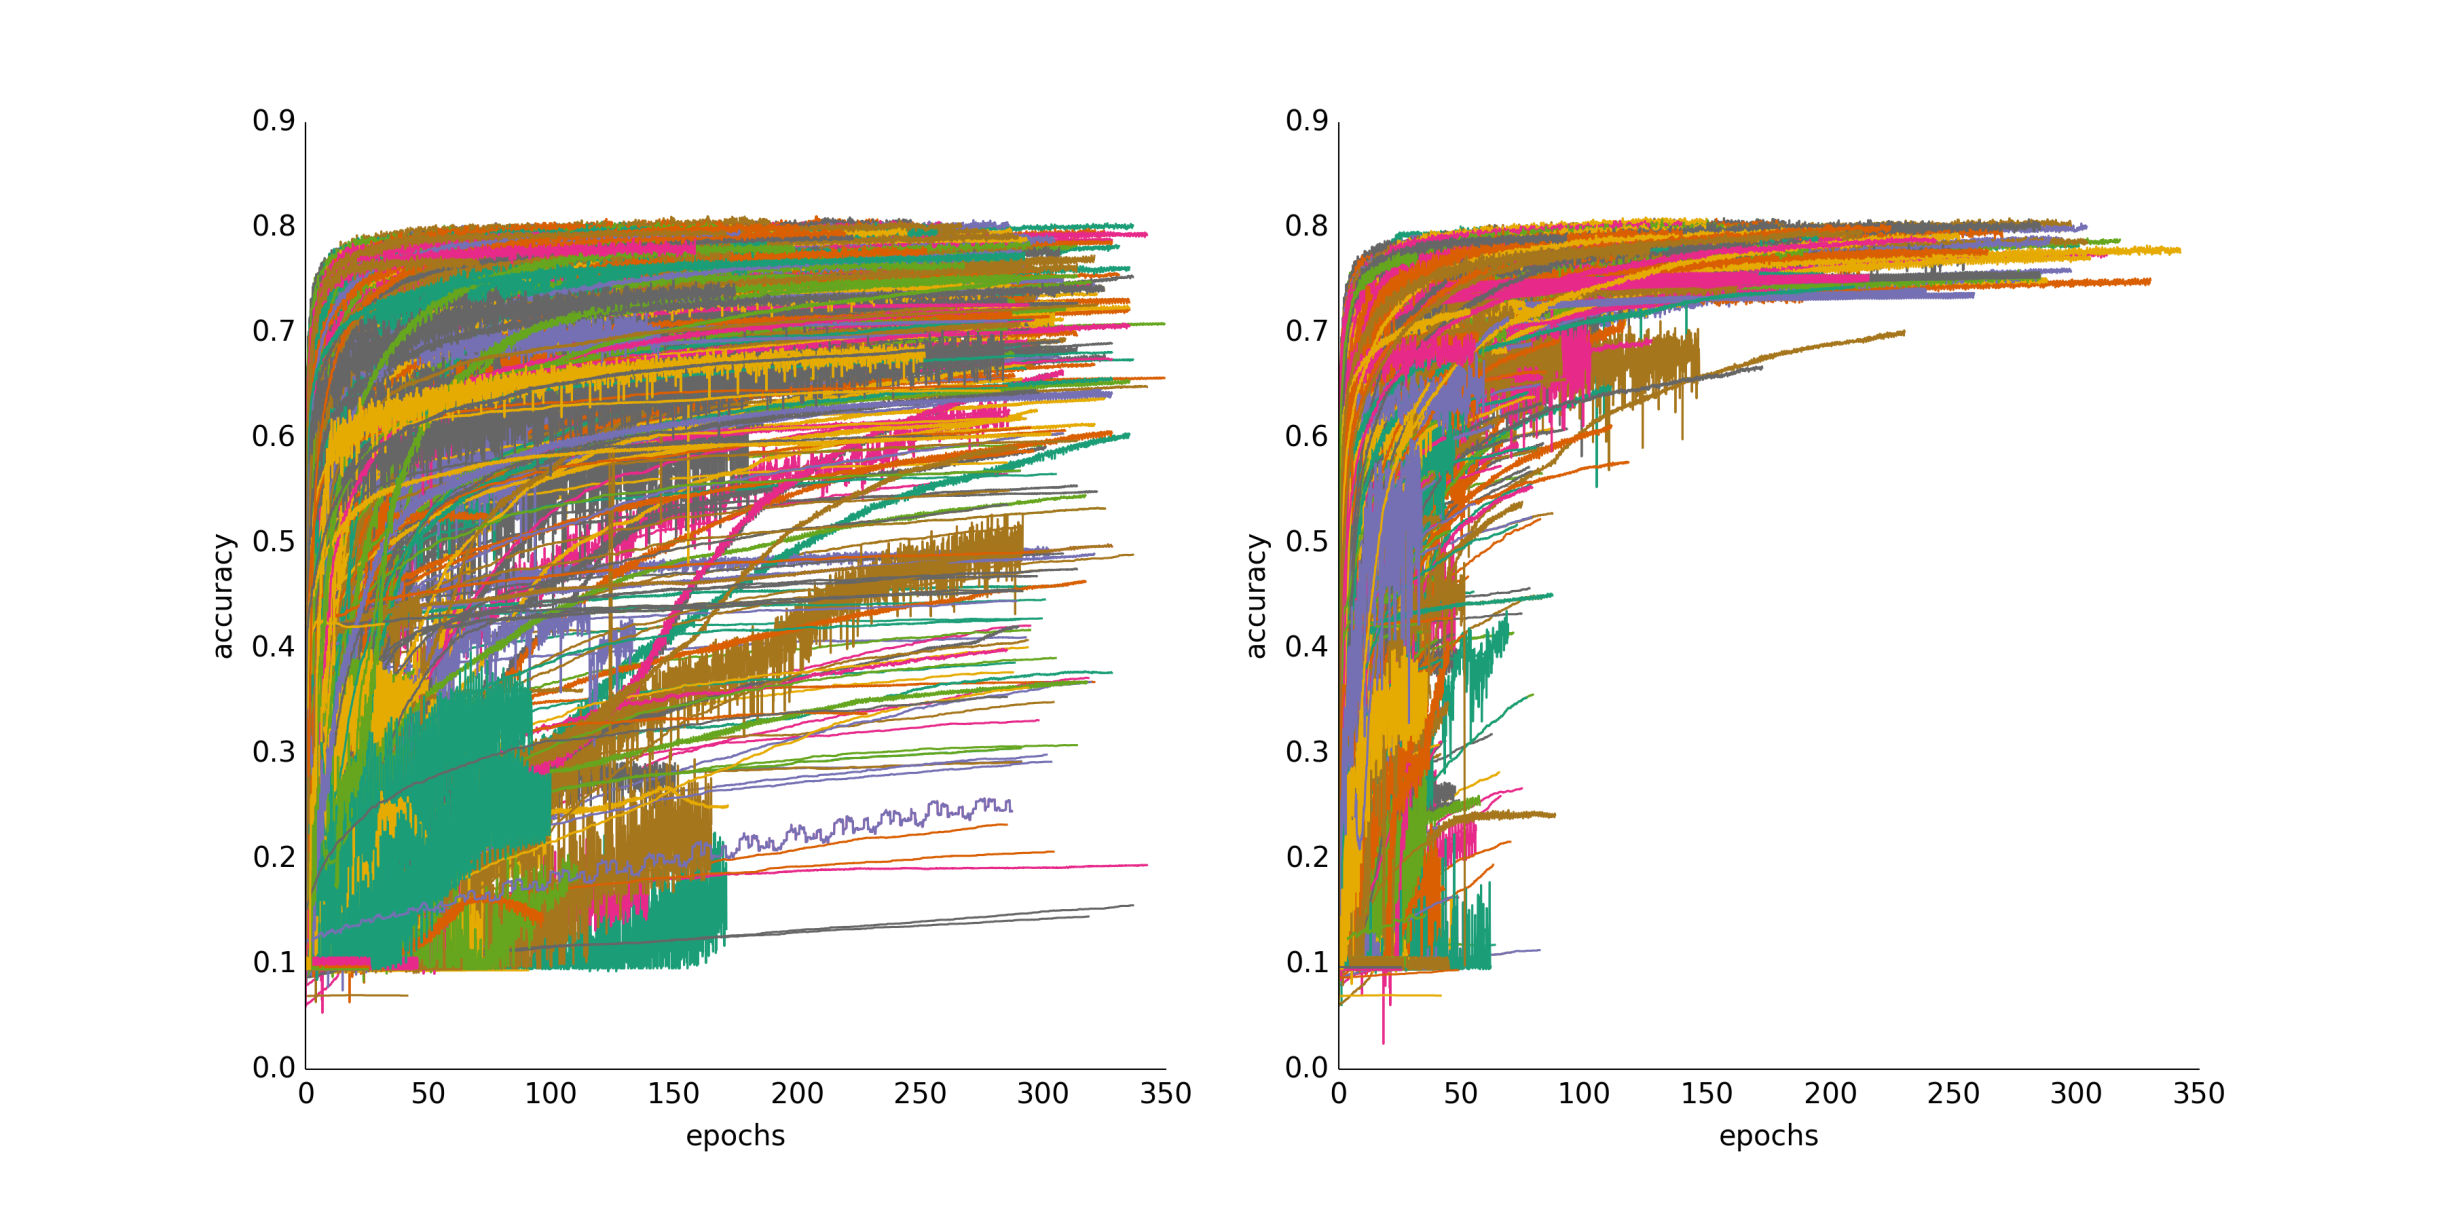
\includegraphics[width=\textwidth]{images/learning_curve_tuning}

All learning curves vs. Learning curves with early termination

\end{frame}
%-----------------------------------------------------------------------

%-----------------------------------------------------------------------
\begin{frame}[c,fragile]{Subset Selection \litw{Klein et al. 2017}}

\begin{itemize}
  \item Problem: training is very slow for large datasets
  \item Idea: scaling up from subsets of data
  \item Example SVM:
  \begin{itemize}
    \item Computational cost grows quadratically in dataset size $s$
    \item Error shrinks smoothly with $s$
    \item Two parameters: $C$, $\lambda$
  \end{itemize}
\end{itemize}

\centering
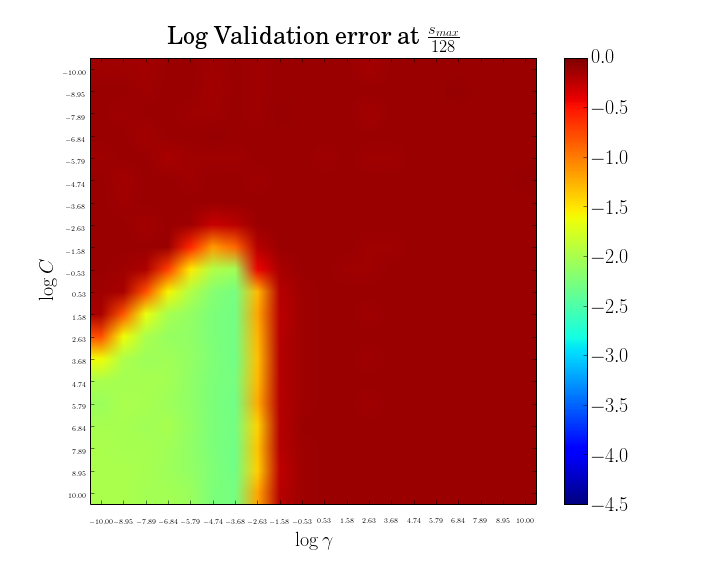
\includegraphics[width=0.28\textwidth]{images/subset_128}
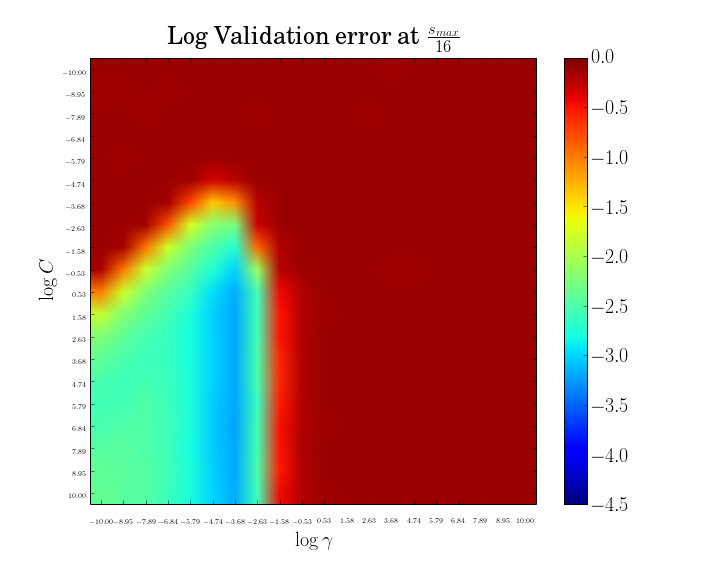
\includegraphics[width=0.28\textwidth]{images/subset_16}\\
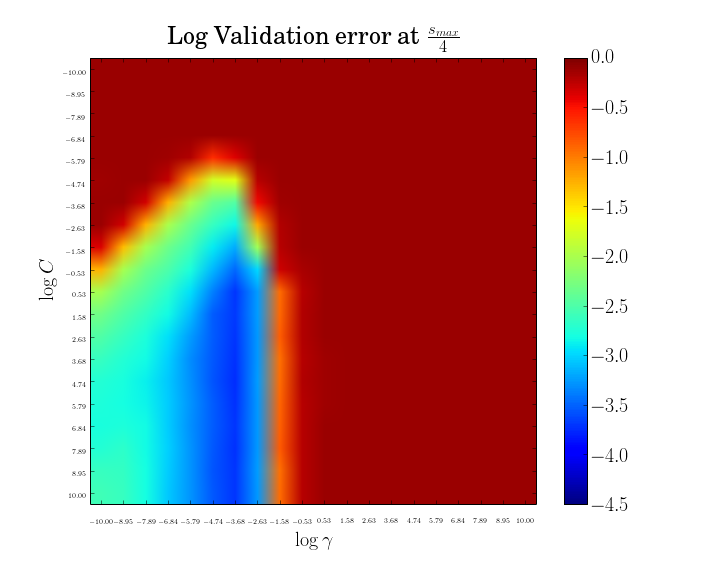
\includegraphics[width=0.28\textwidth]{images/subset_4}
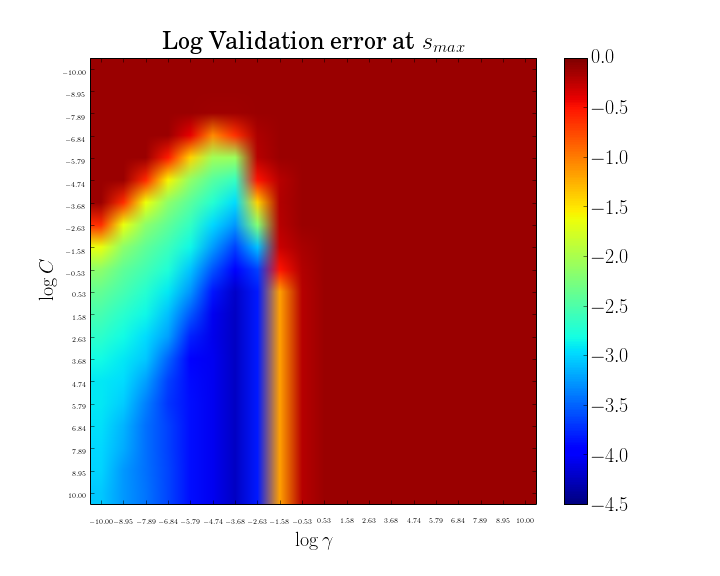
\includegraphics[width=0.28\textwidth]{images/subset_full}


\end{frame}
%-----------------------------------------------------------------------

%-----------------------------------------------------------------------
\begin{frame}[c,fragile]{Subset Selection \litw{Klein et al. 2017}}

\begin{itemize}
  \item Automatically choose dataset size for each evaluation
  \item Include extra dimension in probabilistic model to capture dependence on dataset size s: $f(\lambda,s)$
  \item Construct a second model for computational cost: $c(\lambda,s)$
  \item Trade off information gain about global optimum vs. cost
  \begin{itemize}
   \item Entropy Search \lit{Hennig & Schuler, JMLR 2012}:\\ Based on a probability distribution of where the maximum lies
  \end{itemize} 
\end{itemize}

\centering
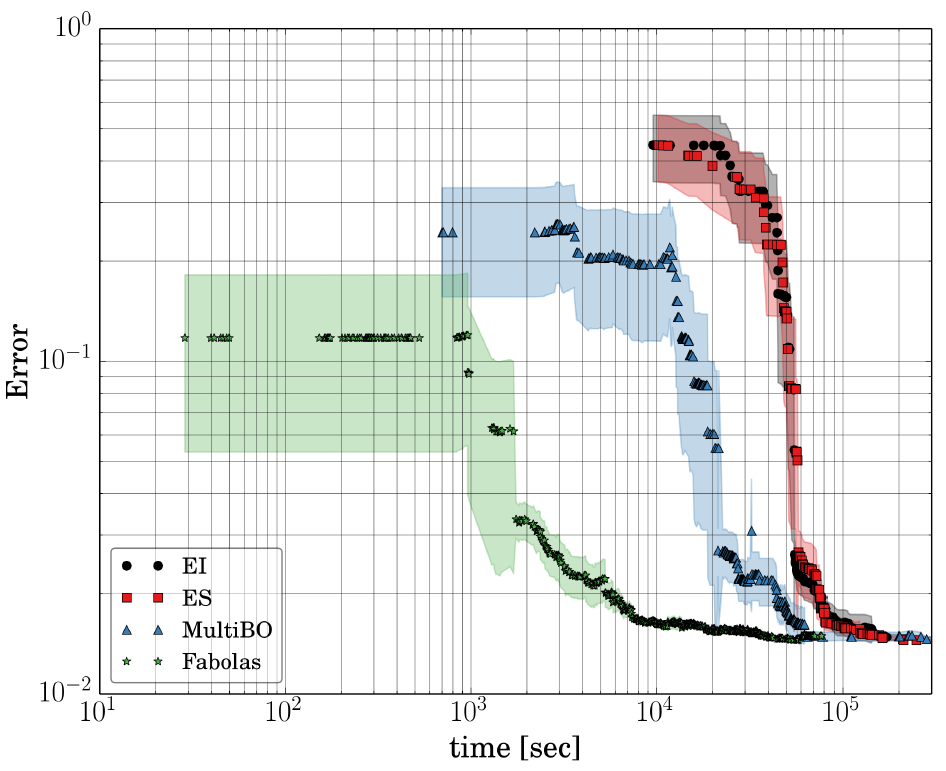
\includegraphics[width=0.4\textwidth]{images/subset_results}

\end{frame}
%-----------------------------------------------------------------------

%-----------------------------------------------------------------------
{\setbeamertemplate{logo}{}
\begin{frame}[c,fragile]{Successive Halving \litw{Jamieson and Talwalkar 2015}}

\begin{block}{Successive Halving}
\begin{itemize}
  \item Ideas: 
  \begin{itemize}
    \item Invest only resources in promising configurations
    \item[$\leadsto$] aggressive dropping of poor configurations
    \item Model-free --- (more or less assumption free)
  \end{itemize}
  \pause
  \item Algorithm Outline:
  \begin{enumerate}
    \item[-] Input: $n$ (randomly sampled) configurations and budget $B$
    \pause
    \item Run remaining configurations with some resource allocation\\ (depending on $B$)
    \pause
    \item Sort configurations by cost (e.$\,$g., validation loss)
    \item Throw away lower half of configurations
    \pause
    \item Repeat
  \end{enumerate}
  \pause
  \item Resource allocation can correspond to
  \begin{itemize}
    \item partial learning curves
    \item subset of training data
  \end{itemize}
\end{itemize}
\end{block}

\end{frame}
}
%-----------------------------------------------------------------------
%-----------------------------------------------------------------------
{\setbeamertemplate{logo}{}
\begin{frame}[c,fragile]{Hyperband \litw{Li et al. 2016}}

\begin{block}{Hyperband}
\begin{itemize}
  \item Issue of successive halving (for a fixed $B$):\\
  		Do you want to run many configurations with aggressive rejection?\\
  		Or: Do you want to run few configurations with non-aggressive rejection? 
  \pause
  \item Ideas: 
  \begin{itemize}
    \item Add an outer loop to try different trade-offs between $\#$configurations and budget
    \item Add further parameter: proportion of configurations discarded in each round of successive halving
  \end{itemize}
  \pause
  \item Starts with many configurations that gets aggressively rejected
  \pause
  \item In later iterations, few configurations with more budget each
  \pause
  \item Returns: configuration with the smallest intermediate loss seen so far.
\end{itemize}
\end{block}

\end{frame}
}
%-----------------------------------------------------------------------
%-----------------------------------------------------------------------
\begin{frame}[c,fragile]{Random Search vs. Hyperband}

\centering
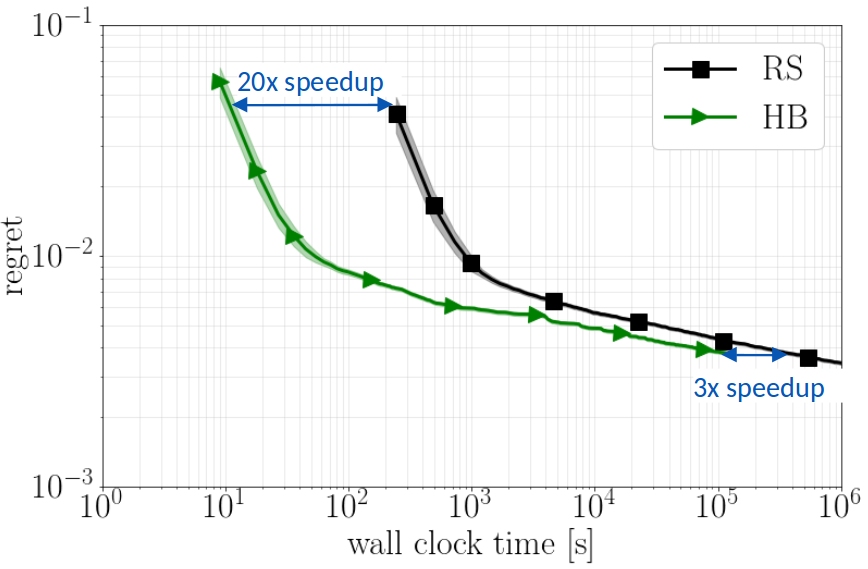
\includegraphics[width=0.8\textwidth]{images/randomsearch_hyperband}

\end{frame}
%-----------------------------------------------------------------------
%-----------------------------------------------------------------------
\begin{frame}[c,fragile]{Random Search vs. Bayesian Optimization}

\centering
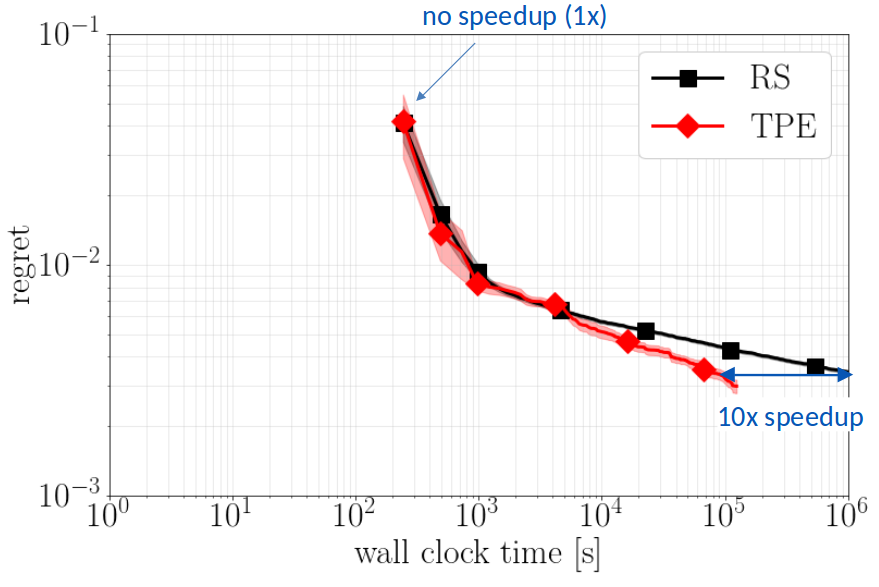
\includegraphics[width=0.8\textwidth]{images/randomsearch_bo}

\end{frame}
%-----------------------------------------------------------------------
%-----------------------------------------------------------------------
\begin{frame}[c,fragile]{Random Search vs. Bayesian Optimization vs. Hyperband}

\centering
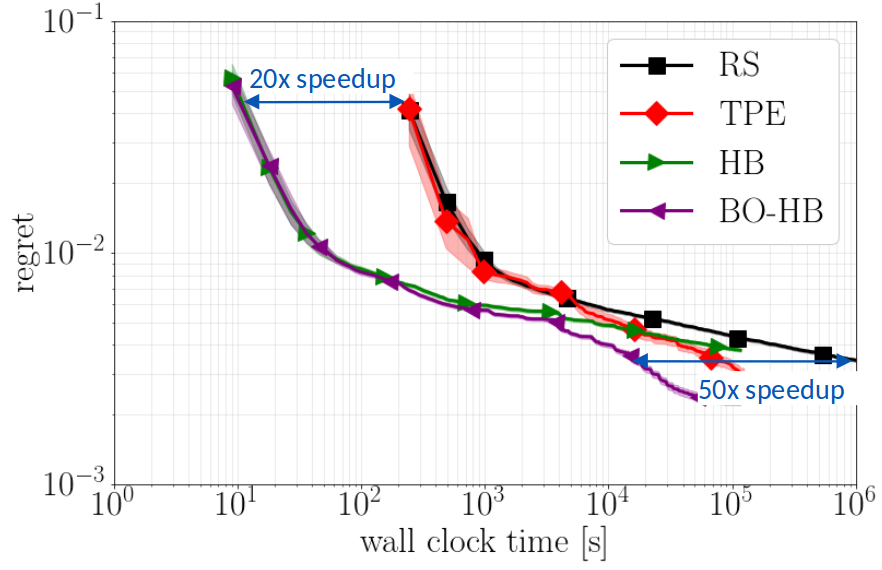
\includegraphics[width=0.8\textwidth]{images/randomsearch_bohb}

\end{frame}
%----------------------------------------------------------------------
%----------------------------------------------------------------------
\begin{frame}[c]{Learning Goals}

After this lecture, you are able to \ldots

\begin{itemize}
	\item explain the \alert{challenges in hyperparameter optimization}
	\item efficiently optimize black box functions via \alert{Bayesian Optimization}
	\begin{itemize}
		\item discuss the advantages of different \alert{surrogate models}
		\item explain the idea of \alert{acquisition functions} to trade off exploration and exploitation
	\end{itemize}
	\item define \alert{configuration spaces}
	\item understand \alert{grey-boxes} for hyperparameter optimization (HPO)
\end{itemize}
\end{frame}
%-----------------------------------------------------------------------